\chapter{Software \& Datasets}
\label{cha:datasets}

\section{Analysis Software}

With the signature of the signal determined, the necessary datasets for the analysis can be chosen. To access and work with these the \textsc{CMSSW} application framework~\cite{cmssw} is used. Aside from providing the analysis tools, the collection of software also contributes to tasks like simulation, calibration, alignment and the event reconstruction. Due to a steady improvement in understanding the detector's and overall experiment's performance, an analysis is also dependent on the version of the \textsc{CMSSW} application framework. This analysis was performed using \verb+CMSSW_5_3_9_patch1+.

Both the simulated and recorded data are stored in the following three data tiers:

\begin{itemize}
\item \textsc{RAW} - This particular format stores the digital information provided by the detector and its system of triggers.
\item \textsc{RECO} - Derived from the \textsc{RAW}-format, the basic event reconstruction has been executed and its results are stored in this format.
\item \textsc{AOD} - Building upon the basic reconstruction, the contents of this format are high level physics objects. This provides most conventional physics analyses, including this one, with the necessary information to base their work upon.
\end{itemize}

By selecting the desired dataset content, the overall size of files can be reduced. For this purpose the \textsc{ACSUSYAnalysis} framework and its skimmer~\cite{acsusyana} are used. This allows for local storage in the form of a tree structure provided by \textsc{ROOT}~\cite{root}. For further analyses and visualization a combination of \textsc{ROOT} version $5.32.00$ and \textsc{findsusyb3}~\cite{findsusyb3} are employed. 


\section{Data}

The four data taking periods from 2012 will be subject of this analysis. The centre-of-mass energy for all of them is $\sqrt{s} = 8\,\text{TeV}$. Since two muons per event are a major part of the signature, the ``DoubleMu'' datasets are the most suitable ones, as they only contain events which activated at least one dimuon trigger. Table~\ref{tab:data} lists the chosen datasets.

\begin{table}[!ht]
  \centering
  \begin{tabular}{|l|c|c|}
    \hline
    Datasets                                         & Run Range         & $\int \mathcal{L} d\text{t}$ [pb$^{-1}$] \\ \hline \hline
    \verb+/DoubleMu/Run2012A-22Jan2013-v1/AOD+\footnotemark       & $190645 - 193621$ & 876                            \\ \hline
    \verb+/DoubleMuParked/Run2012B-22Jan2013-v1/AOD+ & $193834 - 196531$ & 4409                           \\ \hline
    \verb+/DoubleMuParked/Run2012C-22Jan2013-v1/AOD+ & $198049 - 203002$ & 7017                           \\ \hline
    \verb+/DoubleMuParked/Run2012D-22Jan2013-v1/AOD+ & $203777 - 208686$ & 7369                           \\ \hline
    $\Sigma$                                         & $190645 - 208686$ & 19671                          \\ \hline
  \end{tabular}
  \caption{Overview of the data recorded by the CMS experiment, which is used in this analysis.}
  \label{tab:data}
\end{table}


Dissecting the full name of a dataset gives different information about its contents. The first part, here DoubleMuParked, hints at the selected particle content. In this case, the \textit{Parked} version superseded the usual DoubleMu datasets by adding an additional offline trigger with a lower transverse momentum threshold. The second part of the name denotes the data taking period and the third one the date at which it was processed. Unless the latter contains ``PromptReco'', the data has since been reprocessed with improved knowledge of the detector, leading to more precise measurements. The datasets which are subject of this analysis are part of the Winter13 ``ReReco'', short for re-reconstruction. The data format, here ``AOD'', is given at the end.

\footnotetext{The DoubleMuParked dataset from the 2012A period is not a superset of the DoubleMu dataset. As such, the DoubleMu dataset is being used, which yields an additional 3\% events in the chosen final state.}

In the second column, the run ranges are listed. Each run is composed of several lumisections with roughly equal duration. In the third column, the integrated luminosity for the individual run ranges is given. It is estimated from the average number $\left< n \right>$ of pixel clusters occurring in the silicon pixel detector (Sec.~\ref{sec:innertracker}) during an inelastic collision~\cite{cms-pixel-lumi-13}.

\begin{equation}
  \label{eq:lumi}
  \mathcal{L} = \frac{\nu \left< n \right>}{\sigma}
\end{equation}

\noindent The frequency of bunch crossings is given by $\nu$ and $\sigma$ denotes the visible cross section. 

In general, only events from the certified list of properly reconstructed events \\ \verb+Cert_190456-208686_8TeV_PromptReco_Collisions12_JSON.txt+\footnote{It is often called the ``golden JSON'' as it is saved in the java script object notation.} are used. The integrated luminosity $\mathcal{L}$ of this list is $19712\,\text{pb}^{-1}$. Comparing it to the sum of all used DoubleMuParked datasets, only a minuscule amount of events ($\sim 0.2\pct$) is not included in this analysis.

\section{Simulation}

As a general concept to differentiate between potential new physics and the standard model processes, this analysis compares the recorded data to simulation. By comparing simulated and measured distributions of observables, more accurately their expected number of events, the probability of a discovery or at least exclusion ranges can be given. Due to the nature of this method, having a precise prediction from the simulation is essential. There is a strong dependence on the knowledge of the relevant standard model processes.

To take the probabilities for the occurrence of the various processes into account, a Monte-Carlo method is used for the simulation. While they describe particle collision physics, the detector simulation is performed with \textsc{GEANT4}~\cite{geant41,geant42}. After simulating the triggers, the events can be reconstructed using the \textsc{CMSSW} application framework.

\begin{table}[htbp!]
  \centering
  \begin{tabular}{|l|r|r|}
    % BEGIN RECEIVE ORGTBL datasetsmc
\hline
Monte Carlo Sample & $\sigma [\text{pb}^{-1}]$ & Weight \\
\hline
\hline
$Z/\gamma^* \rightarrow ll$ $(10\,\text{GeV} < m_{ll} < 50\,\text{GeV})$ & 762 & $1.25 \cdot 2.10$ \\
$Z/\gamma^* \rightarrow ll$ $(50\,\text{GeV} < m_{ll})$ & $3.50 \cdot 10^3$ $\star$$\star$ & $0.96 \cdot 2.26$ \\
\hline
QCD $\mu_{p_\text{T} > 5\,\text{GeV}}$-enr. ($15\,\text{GeV} < \hat{p}_{\text{T}} < 20\,\text{GeV}$) & $2.74 \cdot 10^6$ & $31.3 \cdot 10^3$ \\
QCD $\mu_{p_\text{T} > 5\,\text{GeV}}$-enr. ($20\,\text{GeV} < \hat{p}_{\text{T}}\footnotemark[3] < 30\,\text{GeV}$) & $1.87 \cdot 10^6$ & $4.32 \cdot 10^3$ \\
QCD $\mu_{p_\text{T} > 5\,\text{GeV}}$-enr. ($30\,\text{GeV} < \hat{p}_{\text{T}} < 50\,\text{GeV}$) & $8.06 \cdot 10^5$ & $1.66 \cdot 10^3$ \\
QCD $\mu_{p_\text{T} > 5\,\text{GeV}}$-enr. ($50\,\text{GeV} < \hat{p}_{\text{T}} < 80\,\text{GeV}$) & $1.76 \cdot 10^5$ & 334 \\
QCD $\mu_{p_\text{T} > 5\,\text{GeV}}$-enr. ($80\,\text{GeV} < \hat{p}_{\text{T}} < 120\,\text{GeV}$) & $4.04 \cdot 10^4$ & 86.1 \\
QCD $\mu_{p_\text{T} > 5\,\text{GeV}}$-enr. ($120\,\text{GeV} < \hat{p}_{\text{T}} < 170\,\text{GeV}$) & $7.46 \cdot 10^3$ & 17.3 \\
QCD $\mu_{p_\text{T} > 5\,\text{GeV}}$-enr. ($170\,\text{GeV} < \hat{p}_{\text{T}} < 300\,\text{GeV}$) & $2.23 \cdot 10^3$ & 5.90 \\
QCD $\mu_{p_\text{T} > 5\,\text{GeV}}$-enr. ($300\,\text{GeV} < \hat{p}_{\text{T}} < 470\,\text{GeV}$) & 151 & 0.381 \\
QCD $\mu_{p_\text{T} > 5\,\text{GeV}}$-enr. ($470\,\text{GeV} < \hat{p}_{\text{T}} < 600\,\text{GeV}$) & 11.8 & 0.0613 \\
QCD $\mu_{p_\text{T} > 5\,\text{GeV}}$-enr. ($600\,\text{GeV} < \hat{p}_{\text{T}} < 800\,\text{GeV}$) & 2.69 & 0.0128 \\
QCD $\mu_{p_\text{T} > 5\,\text{GeV}}$-enr. ($800\,\text{GeV} < \hat{p}_{\text{T}} < 1000\,\text{GeV}$) & 0.369 & 0.0018 \\
QCD $\mu_{p_\text{T} > 5\,\text{GeV}}$-enr. ($1000\,\text{GeV} < \hat{p}_{\text{T}}$) & 0.0849 & 0.0004 \\
\hline
$t^+$ ($s$-channel) & $3.79 \pm 0.7$ $\star$$\star$$\star$ \cite{topxsec} & 0.532 \\
$t^-$ ($s$-channel) & $1.76 \pm 0.01$ $\star$$\star$$\star$ \cite{topxsec} & 0.133 \\
$t^+$ ($t$-channel) & $56.4^{+ 2.1}_{- 0.3}$ $\star$$\star$$\star$ \cite{topxsec} & 0.573 \\
$t^-$ ($t$-channel) & $30.7 \pm 0.7$ $\star$$\star$$\star$ \cite{topxsec} & 6.05 \\
$t^+$ ($tW$-channel) & $11.1 \pm 0.3$ $\star$$\star$$\star$ \cite{topxsec} & 0.555 \\
$t^-$ ($tW$-channel) & $11.1 \pm 0.3$ $\star$$\star$$\star$ \cite{topxsec} & 0.439 \\
\hline
$t\bar{t}$ \footnotemark[4] & $234^{+10}_{-9}$ $\star$$\star$$\star$ & 0.212 \\
\hline
$t\bar{t} + W$ & $0.232 \pm 0.067$ $\star$ & 0.0210 \\
$t\bar{t} + WW$ & 0.002037 & 0.0002 \\
$t\bar{t} + Z$ & $0.2057^{+0.019}_{-0.024}$ & 0.0193 \\
\hline
$W + \text{jets} \rightarrow l + \nu$ & $3.75 \cdot 10^4$$\star$$\star$ & 12.8 \\
\hline
$W + \gamma \rightarrow l + \nu + 2 \mu$ \footnotemark[4] & 1.91 & 0.126 \\
$WW + \text{jets} \rightarrow 2 l + 2 \nu$ & $5.885 \pm 0.396$ $\star$ & 0.0599 \\
$WZ + \text{jets} \rightarrow 2 l + 2 q$ & $2.293 \pm 0.126$ $\star$ & 0.0140 \\
$WZ + \text{jets} \rightarrow 2 q + l \nu$ & $7.495 \pm 0.455$ $\star$ & 0.0507 \\
$WZ + \text{jets} \rightarrow 3 l + \nu$ & $1.105 \pm 0.066$ $\star$ & 0.0108 \\
$ZZ + \text{jets} \rightarrow 2 l + 2 \nu$ & $0.358 \pm 0.019$ $\star$ & 0.0074 \\
$ZZ + \text{jets} \rightarrow 2 l + 2 q$ & $1.251 \pm 0.065$ $\star$ & 0.0127 \\
$ZZ + \text{jets} \rightarrow 4 l$ & $0.181 \pm 0.009$ $\star$ & 0.0007 \\
\hline
$WWW$ & $0.08068^{+4.7\,\pct}_{-3.9\,\pct}$ $\star$ & 0.0072 \\
$WWZ$ & $0.0580^{+5.6\,\pct}_{-4.6\,\pct}$ $\star$ & 0.0051 \\
$WZZ$ & $0.0197^{+6.0\,\pct}_{-4.9\,\pct}$ $\star$ & 0.0018 \\
$ZZZ$ & $0.00553^{+2.7\,\pct}_{-2.4\,\pct}$ $\star$ & 0.0005 \\
\hline
$W^-W^-$ & 0.0889 & 0.0181 \\
$W^+W^+$ & 0.248 & 0.0488 \\
$WW$-DoubleParton & 0.588 & 0.0139 \\
\hline
    % END RECEIVE ORGTBL datasetsmc
  \end{tabular}
  \caption{List of all Monte Carlo samples that are considered as backgrounds for this analysis. Leading order cross sections are unmarked, while the stars indicate NLO ($\star$), NNLO($\star$$\star$) and approx. NNLO($\star$$\star$$\star$) calculations. Unless noted otherwise, the LO cross sections are taken from the generator output and the higher order ones including their scale uncertainties (if given) are from~\cite{xsec}.}
  \label{tab:mcsamples}
\end{table}

\footnotetext[3]{$\hat{p}_{\text{T}}$ refers transverse momentum of the hard interaction.} 
\footnotetext[4]{\textsc{Pythia6} does not include $W$ and $Z$ bosons in the showering process, which is why additional $t\bar{t} + V$ samples are required. This also applies to the $\gamma \rightarrow \mu\mu$ decay in the $W + \text{jets} \rightarrow l \nu$ process.} 


\begin{comment}
  #+ORGTBL: SEND datasetsmc orgtbl-to-latex :splice t :no-escape t
  |--------------------------------------------------------------------------------------------------------------------+-------------------------------------------------------------+-------------------|
  | Monte Carlo Sample                                                                                                 | $\sigma [\text{pb}^{-1}]$                                   |            Weight |
  |--------------------------------------------------------------------------------------------------------------------+-------------------------------------------------------------+-------------------|
  |--------------------------------------------------------------------------------------------------------------------+-------------------------------------------------------------+-------------------|
  | $Z/\gamma^* \rightarrow ll$ $(10\,\text{GeV} < m_{ll} < 50\,\text{GeV})$                                           | 762                                                         | $1.25 \cdot 2.10$ |
  | $Z/\gamma^* \rightarrow ll$ $(50\,\text{GeV} < m_{ll})$                                                            | $3.50 \cdot 10^3$ $\star$$\star$                            | $0.96 \cdot 2.26$ |
  |--------------------------------------------------------------------------------------------------------------------+-------------------------------------------------------------+-------------------|
  | QCD $\mu_{p_\text{T} > 5\,\text{GeV}}$-enr. ($15\,\text{GeV} < \hat{p}_{\text{T}} < 20\,\text{GeV}$)               | $2.74 \cdot 10^6$                                           | $31.3 \cdot 10^3$ |
  | QCD $\mu_{p_\text{T} > 5\,\text{GeV}}$-enr. ($20\,\text{GeV} < \hat{p}_{\text{T}} \footnotemark[3] < 30\,\text{GeV}$) | $1.87 \cdot 10^6$                                           | $4.32 \cdot 10^3$ |
  | QCD $\mu_{p_\text{T} > 5\,\text{GeV}}$-enr. ($30\,\text{GeV} < \hat{p}_{\text{T}} < 50\,\text{GeV}$)               | $8.06 \cdot 10^5$                                           | $1.66 \cdot 10^3$ |
  | QCD $\mu_{p_\text{T} > 5\,\text{GeV}}$-enr. ($50\,\text{GeV} < \hat{p}_{\text{T}} < 80\,\text{GeV}$)               | $1.76 \cdot 10^5$                                           |               334 |
  | QCD $\mu_{p_\text{T} > 5\,\text{GeV}}$-enr. ($80\,\text{GeV} < \hat{p}_{\text{T}} < 120\,\text{GeV}$)              | $4.04 \cdot 10^4$                                           |              86.1 |
  | QCD $\mu_{p_\text{T} > 5\,\text{GeV}}$-enr. ($120\,\text{GeV} < \hat{p}_{\text{T}} < 170\,\text{GeV}$)             | $7.46 \cdot 10^3$                                           |              17.3 |
  | QCD $\mu_{p_\text{T} > 5\,\text{GeV}}$-enr. ($170\,\text{GeV} < \hat{p}_{\text{T}} < 300\,\text{GeV}$)             | $2.23 \cdot 10^3$                                           |              5.90 |
  | QCD $\mu_{p_\text{T} > 5\,\text{GeV}}$-enr. ($300\,\text{GeV} < \hat{p}_{\text{T}} < 470\,\text{GeV}$)             | 151                                                         |             0.381 |
  | QCD $\mu_{p_\text{T} > 5\,\text{GeV}}$-enr. ($470\,\text{GeV} < \hat{p}_{\text{T}} < 600\,\text{GeV}$)             | 11.8                                                        |            0.0613 |
  | QCD $\mu_{p_\text{T} > 5\,\text{GeV}}$-enr. ($600\,\text{GeV} < \hat{p}_{\text{T}} < 800\,\text{GeV}$)             | 2.69                                                        |            0.0128 |
  | QCD $\mu_{p_\text{T} > 5\,\text{GeV}}$-enr. ($800\,\text{GeV} < \hat{p}_{\text{T}} < 1000\,\text{GeV}$)            | 0.369                                                       |            0.0018 |
  | QCD $\mu_{p_\text{T} > 5\,\text{GeV}}$-enr. ($1000\,\text{GeV} < \hat{p}_{\text{T}}$)                              | 0.0849                                                      |            0.0004 |
  |--------------------------------------------------------------------------------------------------------------------+-------------------------------------------------------------+-------------------|
  | $t^+$ ($s$-channel)                                                                                                | $3.79 \pm 0.7$ $\star$$\star$$\star$ \cite{topxsec}         |             0.532 |
  | $t^-$ ($s$-channel)                                                                                                | $1.76 \pm 0.01$ $\star$$\star$$\star$ \cite{topxsec}        |             0.133 |
  | $t^+$ ($t$-channel)                                                                                                | $56.4^{+ 2.1}_{- 0.3}$ $\star$$\star$$\star$ \cite{topxsec} |             0.573 |
  | $t^-$ ($t$-channel)                                                                                                | $30.7 \pm 0.7$ $\star$$\star$$\star$ \cite{topxsec}         |              6.05 |
  | $t^+$ ($tW$-channel)                                                                                               | $11.1 \pm 0.3$ $\star$$\star$$\star$ \cite{topxsec}         |             0.555 |
  | $t^-$ ($tW$-channel)                                                                                               | $11.1 \pm 0.3$ $\star$$\star$$\star$ \cite{topxsec}         |             0.439 |
  |--------------------------------------------------------------------------------------------------------------------+-------------------------------------------------------------+-------------------|
  | $t\bar{t}$ \footnotemark[4]                                                                                          | $234^{+10}_{-9}$ $\star$$\star$$\star$                      |             0.212 |
  |--------------------------------------------------------------------------------------------------------------------+-------------------------------------------------------------+-------------------|
  | $t\bar{t} + W$                                                                                                     | $0.232 \pm 0.067$ $\star$                                   |            0.0210 |
  | $t\bar{t} + WW$                                                                                                    | 0.002037                                                    |            0.0002 |
  | $t\bar{t} + Z$                                                                                                     | $0.2057^{+0.019}_{-0.024}$                                  |            0.0193 |
  |--------------------------------------------------------------------------------------------------------------------+-------------------------------------------------------------+-------------------|
  | $W + \text{jets} \rightarrow l + \nu$                                                                              | $3.75 \cdot 10^4$$\star$$\star$                             |              12.8 |
  |--------------------------------------------------------------------------------------------------------------------+-------------------------------------------------------------+-------------------|
  | $W + \gamma \rightarrow l + \nu + 2 \mu$ \footnotemark[4]                                                                           | 1.91                                                        |             0.126 |
  | $WW + \text{jets} \rightarrow 2 l + 2 \nu$                                                                         | $5.885 \pm 0.396$ $\star$                                   |            0.0599 |
  | $WZ + \text{jets} \rightarrow 2 l + 2 q$                                                                           | $2.293 \pm 0.126$ $\star$                                   |            0.0140 |
  | $WZ + \text{jets} \rightarrow 2 q + l \nu$                                                                         | $7.495 \pm 0.455$ $\star$                                   |            0.0507 |
  | $WZ + \text{jets} \rightarrow 3 l + \nu$                                                                           | $1.105 \pm 0.066$ $\star$                                   |            0.0108 |
  | $ZZ + \text{jets} \rightarrow 2 l + 2 \nu$                                                                         | $0.358 \pm 0.019$ $\star$                                   |            0.0074 |
  | $ZZ + \text{jets} \rightarrow 2 l + 2 q$                                                                           | $1.251 \pm 0.065$ $\star$                                   |            0.0127 |
  | $ZZ + \text{jets} \rightarrow 4 l$                                                                                 | $0.181 \pm 0.009$ $\star$                                   |            0.0007 |
  |--------------------------------------------------------------------------------------------------------------------+-------------------------------------------------------------+-------------------|
  | $WWW$                                                                                                              | $0.08068^{+4.7\,\pct}_{-3.9\,\pct}$ $\star$                 |            0.0072 |
  | $WWZ$                                                                                                              | $0.0580^{+5.6\,\pct}_{-4.6\,\pct}$ $\star$                  |            0.0051 |
  | $WZZ$                                                                                                              | $0.0197^{+6.0\,\pct}_{-4.9\,\pct}$ $\star$                  |            0.0018 |
  | $ZZZ$                                                                                                              | $0.00553^{+2.7\,\pct}_{-2.4\,\pct}$ $\star$                 |            0.0005 |
  |--------------------------------------------------------------------------------------------------------------------+-------------------------------------------------------------+-------------------|
  | $W^-W^-$                                                                                                           | 0.0889                                                      |            0.0181 |
  | $W^+W^+$                                                                                                           | 0.248                                                       |            0.0488 |
  | $WW$-DoubleParton                                                                                                  | 0.588                                                       |            0.0139 |
  |--------------------------------------------------------------------------------------------------------------------+-------------------------------------------------------------+-------------------|
\end{comment}

All Standard Model samples that can produce two muons and two jets are considered as backgrounds for this analysis are given in table~\ref{tab:mcsamples}. The samples were generated during the ``Summer12'' period using \textsc{Pythia6}~\cite{pythia6} for QCD, \textsc{Powheg}~\cite{powheg,powhegst,powhegtt} for single and pair production of top-quarks and \textsc{Madgraph}~\cite{madgraph5} for most others. Details can be extracted from the sample paths, which are given in appendix~\ref{cha:mcsamppath}. In columns two and three, the cross section and weight of the specific processes are given. The latter is necessary to adjust the generated number of events for each sample to the expected amount for a given luminosity. Producing Monte Carlos samples individually for each analysis would not only be inefficient, but also very resource intensive. Instead most samples are produced centrally, which is also the reason why the generated and expected number of events cannot be matched. The formula for calculating the weight is

\begin{equation}
  \label{eq:weight}
  w = f \cdot \frac{\sigma \cdot \mathcal{L}_{\text{int}}}{N}.
\end{equation}

\noindent The variable parameters are the cross section $\sigma$ and the number of generated events $N$. The value for the integrated luminosity $\mathcal{L}_{\text{int}}$ is given by the $19.7\,\text{fb}^{-1}$ that is being used. An additional scaling factor $f$ can be introduced to account for effects like higher order corrections to a cross section. It is only employed for the Drell-Yan processes and is listed in the weights column of table~\ref{tab:mcsamples}. The first factor of the product is $f$. The way these scaling factors are determined is described in an upcoming section (Sec.~\ref{sec:scaling}).

In all following distributions, groups of backgrounds are summarized under a single title to avoid cluttering. Table~\ref{tab:mcpooltitles} lists the names which will be used.

\begin{table}[!htb]
  \centering
  \begin{tabular}{|l|l|}
    % BEGIN RECEIVE ORGTBL mcpooltitles
\hline
Title & Monte Carlo Samples \\
\hline
Drell-Yan & Both $Z/\gamma^* \rightarrow ll$ \\
QCD & All QCD samples \\
Single-top & $t^\pm$ $s$-, $t$- and $tW$-channels \\
$t \bar{t}$ & $t \bar{t}$ \\
$t \bar{t} + V$ & $t \bar{t} + W$, $t \bar{t} + WW$ and $t \bar{t} + Z$ \\
$W \rightarrow l \nu$ & $W + \text{jets} \rightarrow l + \nu$ \\
DiBoson & $W\gamma$ and all $WW$, $WZ$, $ZZ$ decay modes \\
$VVV$ & $WWW$, $WWZ$, $WZZ$ and $ZZZ$ \\
Rare Samples & $W^-W^-$, $W^+W^+$ and $WW$-DoubleParton \\
\hline
    % END RECEIVE ORGTBL mcpooltitles    
  \end{tabular}
  \caption{Arrangement of Monte Carlo titles in the distributions. Under each name on the left, the corresponding samples on the right are summarized.}
  \label{tab:mcpooltitles}
\end{table}
\begin{comment}
  #+ORGTBL: SEND mcpooltitles orgtbl-to-latex :splice t :skip 0 :no-escape t
  |-----------------------+-----------------------------------------------------------------------------|
  | Title                 | Monte Carlo Samples                                                         |
  |-----------------------+-----------------------------------------------------------------------------|
  | Drell-Yan             | Both $Z/\gamma^* \rightarrow ll$                                            |
  | QCD                   | All QCD samples                                                             |
  | Single-top            | $t^\pm$ $s$-, $t$- and $tW$-channels                                        |
  | $t \bar{t}$           | $t \bar{t}$                                                                 |
  | $t \bar{t} + V$       | $t \bar{t} + W$, $t \bar{t} + WW$ and $t \bar{t} + Z$ |
  | $W \rightarrow l \nu$ | $W + \text{jets} \rightarrow l + \nu$                                       |
  | DiBoson               | $W\gamma$ and all $WW$, $WZ$, $ZZ$ decay modes                              |
  | $VVV$                 | $WWW$, $WWZ$, $WZZ$ and $ZZZ$                                               |
  | Rare Samples          | $W^-W^-$, $W^+W^+$ and $WW$-DoubleParton                                    |
  |-----------------------+-----------------------------------------------------------------------------|
\end{comment}

\begin{figure}[htb!]
  \centering
  \begin{subfigure}[b]{0.495\textwidth}
    \centering
    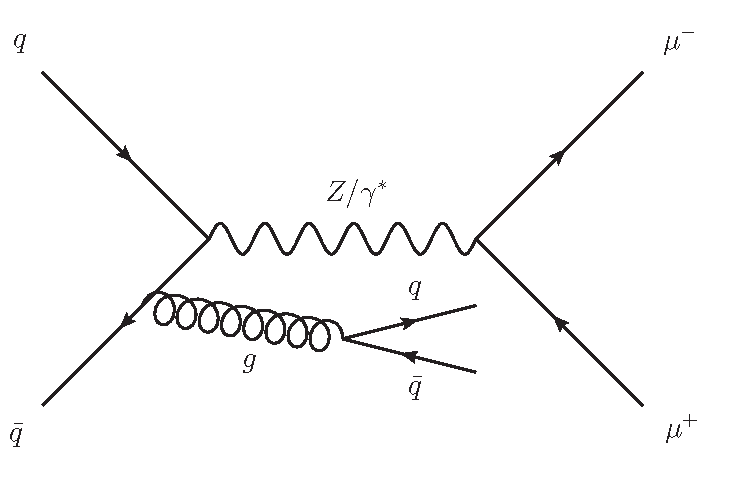
\includegraphics[width=\textwidth]{plots/dyll.pdf}
    \caption{\label{fig:dyll}}
  \end{subfigure}
  \begin{subfigure}[b]{0.495\textwidth}
    \centering
    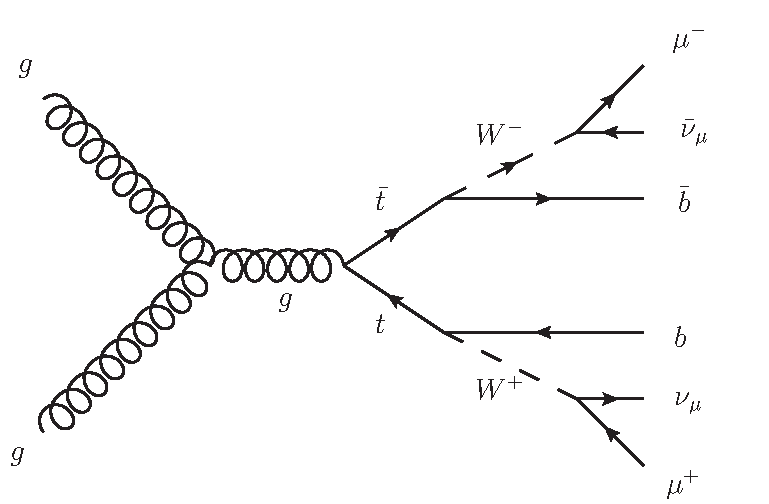
\includegraphics[width=\textwidth]{plots/ttbar.pdf}
    \caption{\label{fig:ttbar}}
  \end{subfigure}
  \caption{Drell-Yan~(\ref{fig:dyll}) and a $t\bar{t}$~(\ref{fig:ttbar}) feynman graph, which lead to a two muon and two jet signature. With their high cross sections, these two processes prove to be dominant Standard Model backgrounds for this analysis. However, they cannot produce two prompt, same sign charge muons.}
  \label{fig:dyllttbar}
\end{figure}

The two Feynman graphs in figure~\ref{fig:dyllttbar} show the dominant background processes. Drell-Yan processes with two muons (Fig.~\ref{fig:dyll}) are the prevalent background before applying the same sign charge requirement. The two lepton final state can provide two muons, although the charge cannot have the same sign. An additional amount of two jets can be produced through radiation of additional bosons or pileup interactions being misinterpreted. After applying the same sign charge requirement, top pair production (Fig.~\ref{fig:ttbar}) becomes the leading Standard Model process. Each top-quark is able to decay via the weak interaction, opening up the possibility of two prompt leptons. However, their charge cannot be equal. Since this analysis requires two prompt, well isolated muons, the ones passing the same sign charge requirement have to have misidentified or mismeasured muon. The likelihood for a muon to be a fake rises with the amount of hadronic activity. All Monte Carlo samples which contribute to the final state due to being dominated by QCD multijet events, will be used to estimate the amount of these contributions.


\subsection{Signal Simulation}
\label{sec:signal-sim}

While the previous section covers the simulation of the standard model background, it is also necessary to generate the supersymmetric model including the signal. In addition to the backgrounds, the simulation of the signal is used to estimate the likelihood of the measurement being described by supersymmetric processes.

To cover a variety of $R$-parity violating constrained MSSM scenarios, the $m_0$-$m_{1/2}$-phase space is subdivided into a grid. The SUSY mass spectra for each point in said grid are generated with \textsc{SoftSusy 3.3.5}~\cite{softsusy,sonnegueth} using the following parameters. The universal mass of scalar particles $m_0$ is increased from $100\,\text{GeV}$ to $2500\,\text{GeV}$ and the universal mass of fermonic ones $m_{1/2}$ from $100\,\text{GeV}$ to $1500\,\text{GeV}$. The size of each step is $100\,\text{GeV}$ for both variables. All remaining parameters are constant throughout the entire grid and are chosen to be

\begin{equation}
  \label{eq:gen-mssm-parameters}
  A_0 = 0, \quad \tan{\beta} = 20, \quad \text{sgn}\,\mu = +1, \quad \lambda^\prime_{211} = 0.01.
\end{equation}

As previously discussed (Cha.~\ref{cha:sig}), certain points in the parameter space do not favour the chosen signal signature while others do yield unphysical results. The former is strictly due the $\tilde{\tau}$-LSP configuration in the high $m_{1/2}$, low $m_0$ region, while the latter has three different reasons. Low values for $m_{1/2}$ and high ones $m_0$ can lead to no electroweak symmetry breaking, non-converging renormalization group equations or the production of tachyons. When generating the mass spectra, all of these scenarios are being excluded before the production. Overall, this leaves $287$ valid points.

To actually produce the events, the leading order matrix element generator \textsc{CalcHep 3.4}~\cite{calchep} is being employed. Generated events are processed with the \textit{full} CMS detector simulation using the \verb+CMSSW_5_3_9_patch1+ framework. The path to the batch file containing all signal samples is also given in appendix~\ref{cha:mcsamppath}. Running the full simulation on the entire grid of parameter points with sufficient statistics for each sample is resource intensive. Therefore a filter is applied at generator level (i.e. before parton showering and simulation) removing events that do not contain at least two muons. They have to pass a transverse momentum threshold of $10\,\text{GeV}$ for the leading muon and $5\,\text{GeV}$ for the sub leading one. These requirements are chosen such that they are well below the \verb+HLT_Mu17_TkMu8+ trigger threshold of $17\,\text{GeV}$ and $8\,\text{GeV}$ for the leading and sub-leading muon, respectively. This filter does not necessitate two muons after the simulation and reconstruction.

In order to increase the accuracy of the \textsc{CalcHep} simulation, $k$-factors are determined as the ratio of a next-to leading order to a leading order cross section calculation. The source code for the NLO calculation is documented in reference~\cite{susyxstool}. They are then applied to the value provided by \textsc{CalcHep}. The branching fractions for the production of the smuon and sneutrino have to be kept in mind. Both the evolution of the smuon's cross section as well as the of $k$-factor are shown in figure~\ref{fig:susys-xs-kfactor}.

\begin{figure}[!htb]
  \centering
  \begin{subfigure}[b]{0.495\textwidth}
    \centering
    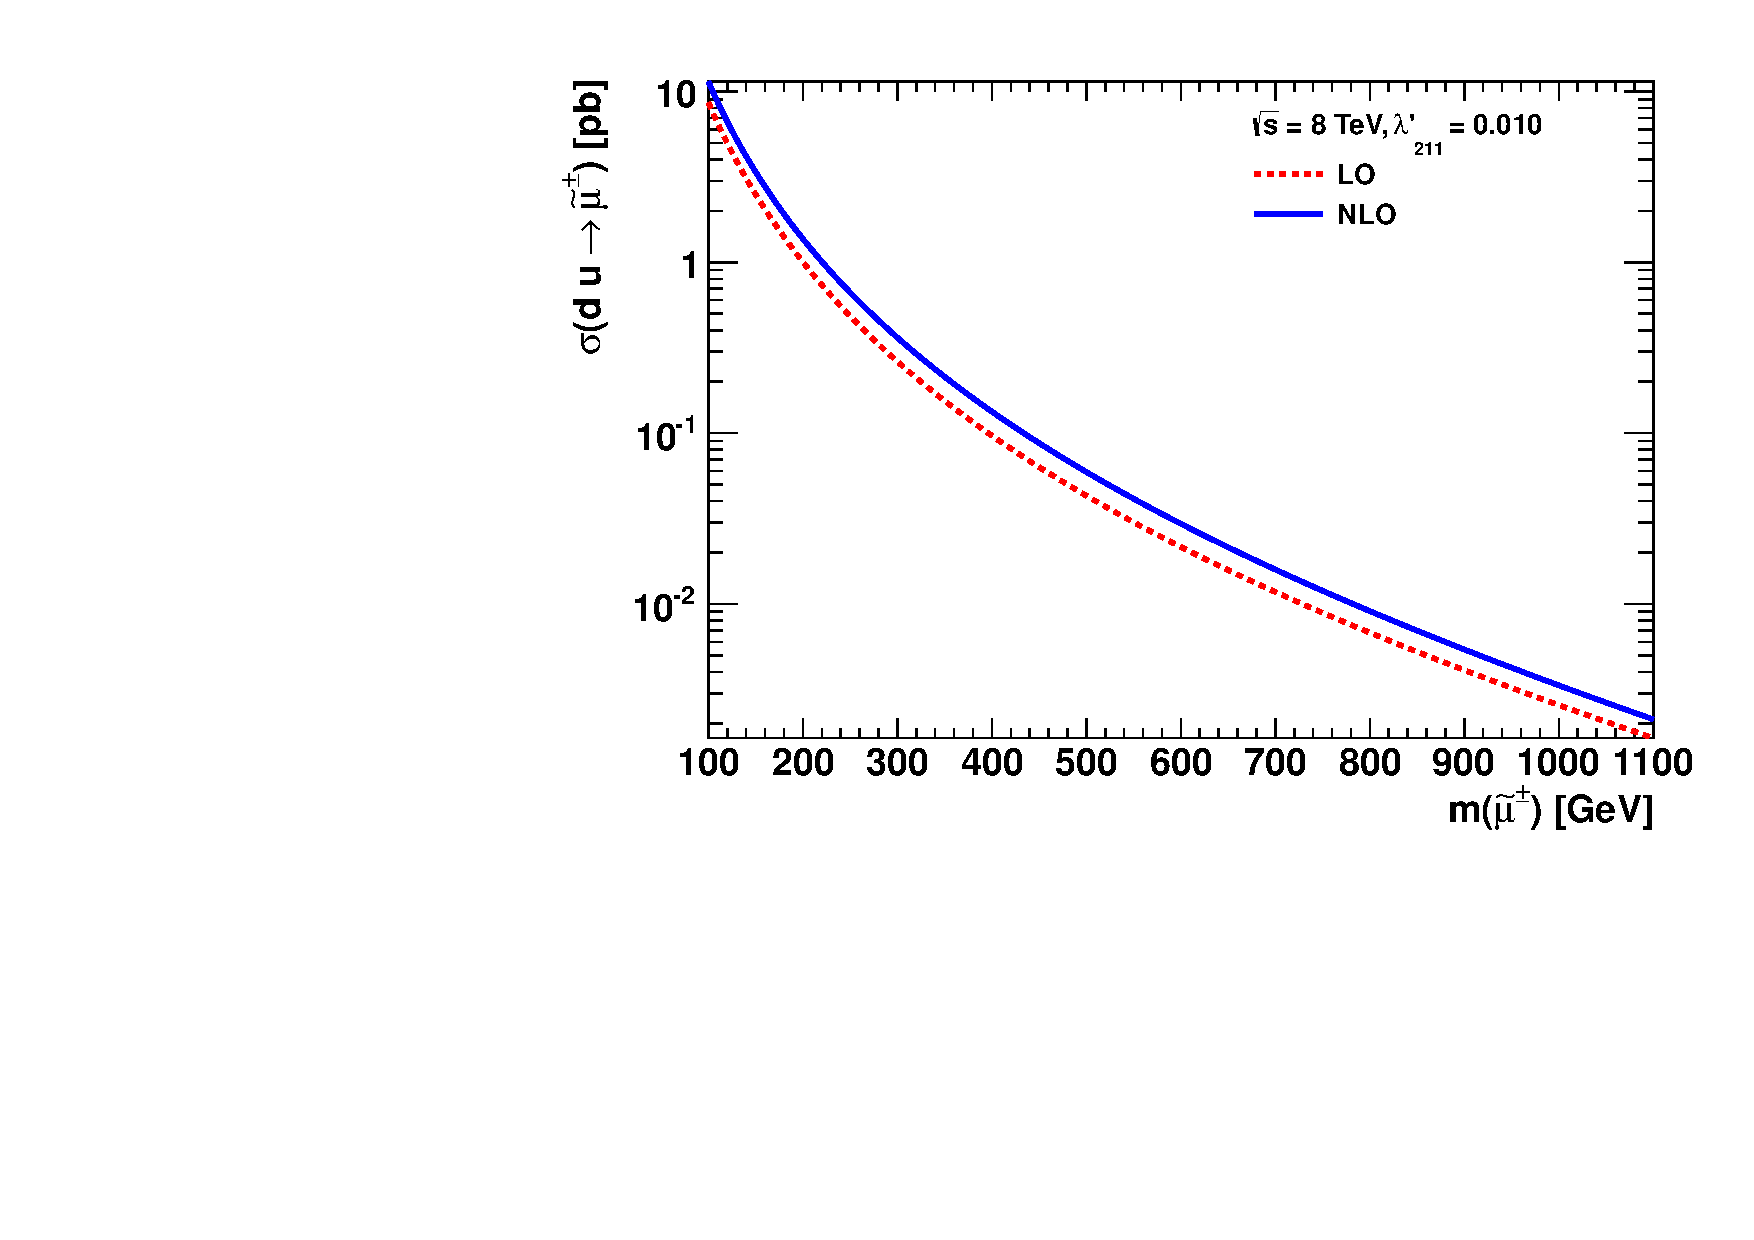
\includegraphics[width=\textwidth]{plots/xs.pdf}
    \caption{\label{fig:xs-smuon}}
  \end{subfigure}
  \begin{subfigure}[b]{0.495\textwidth}
    \centering
    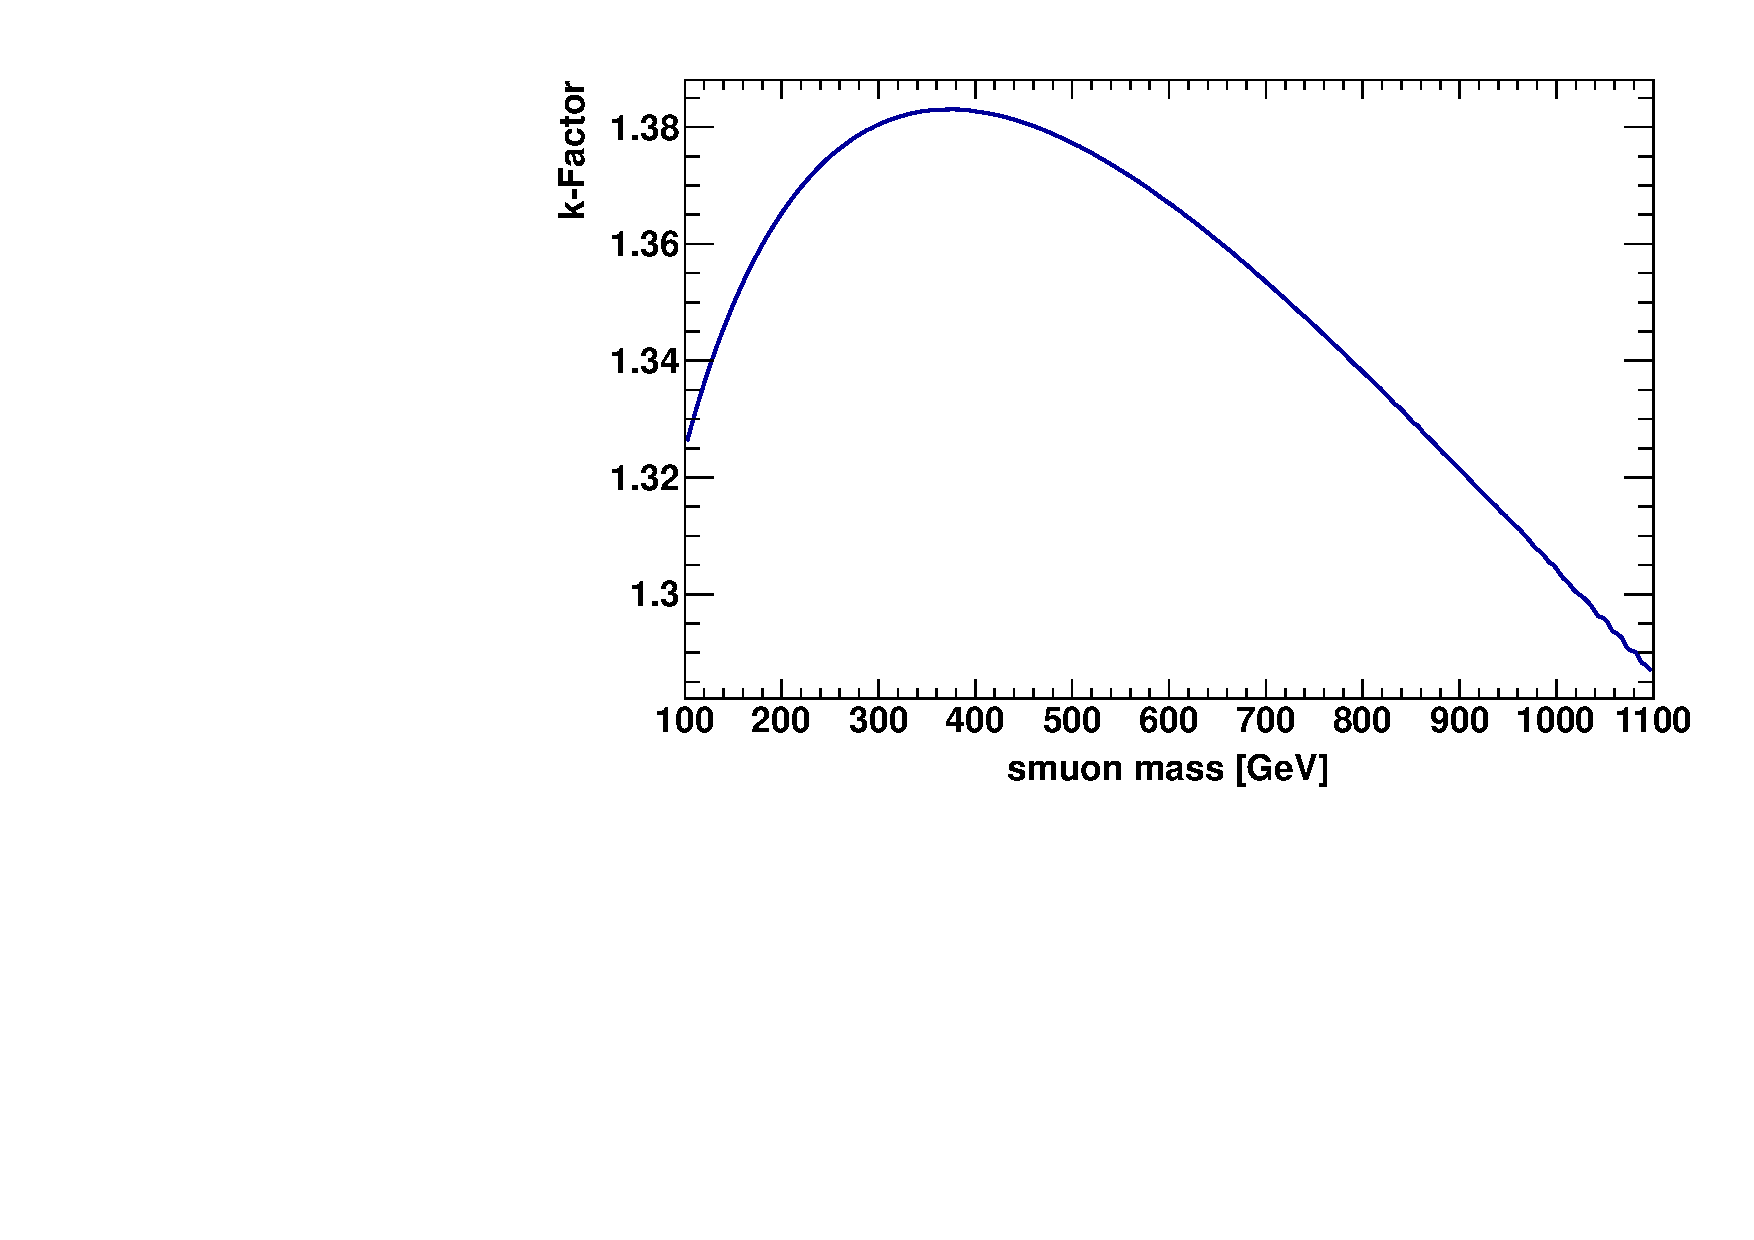
\includegraphics[width=\textwidth]{plots/k_smuon.pdf}
    \caption{\label{fig:k-smuon}}
  \end{subfigure}
  \caption{Cross section for the production of smuons via $\lambda^\prime_{211}$ (\ref{fig:xs-smuon}) and the $k$-factor for their cross section (\ref{fig:k-smuon}). The latter is the ratio of the LO and NLO cross section with respect to the smuons production rate.}
  \label{fig:susys-xs-kfactor}
\end{figure}

\noindent Applying the $k$-factors to the \textsc{CalcHep} output, with respect to the production rate of the smuon and sneutrino, yields the map of next-to leading orders cross sections used in the analysis. This map is shown in figure~\ref{fig:susy-2dxs}.

\begin{figure}[!htb]
  \centering
  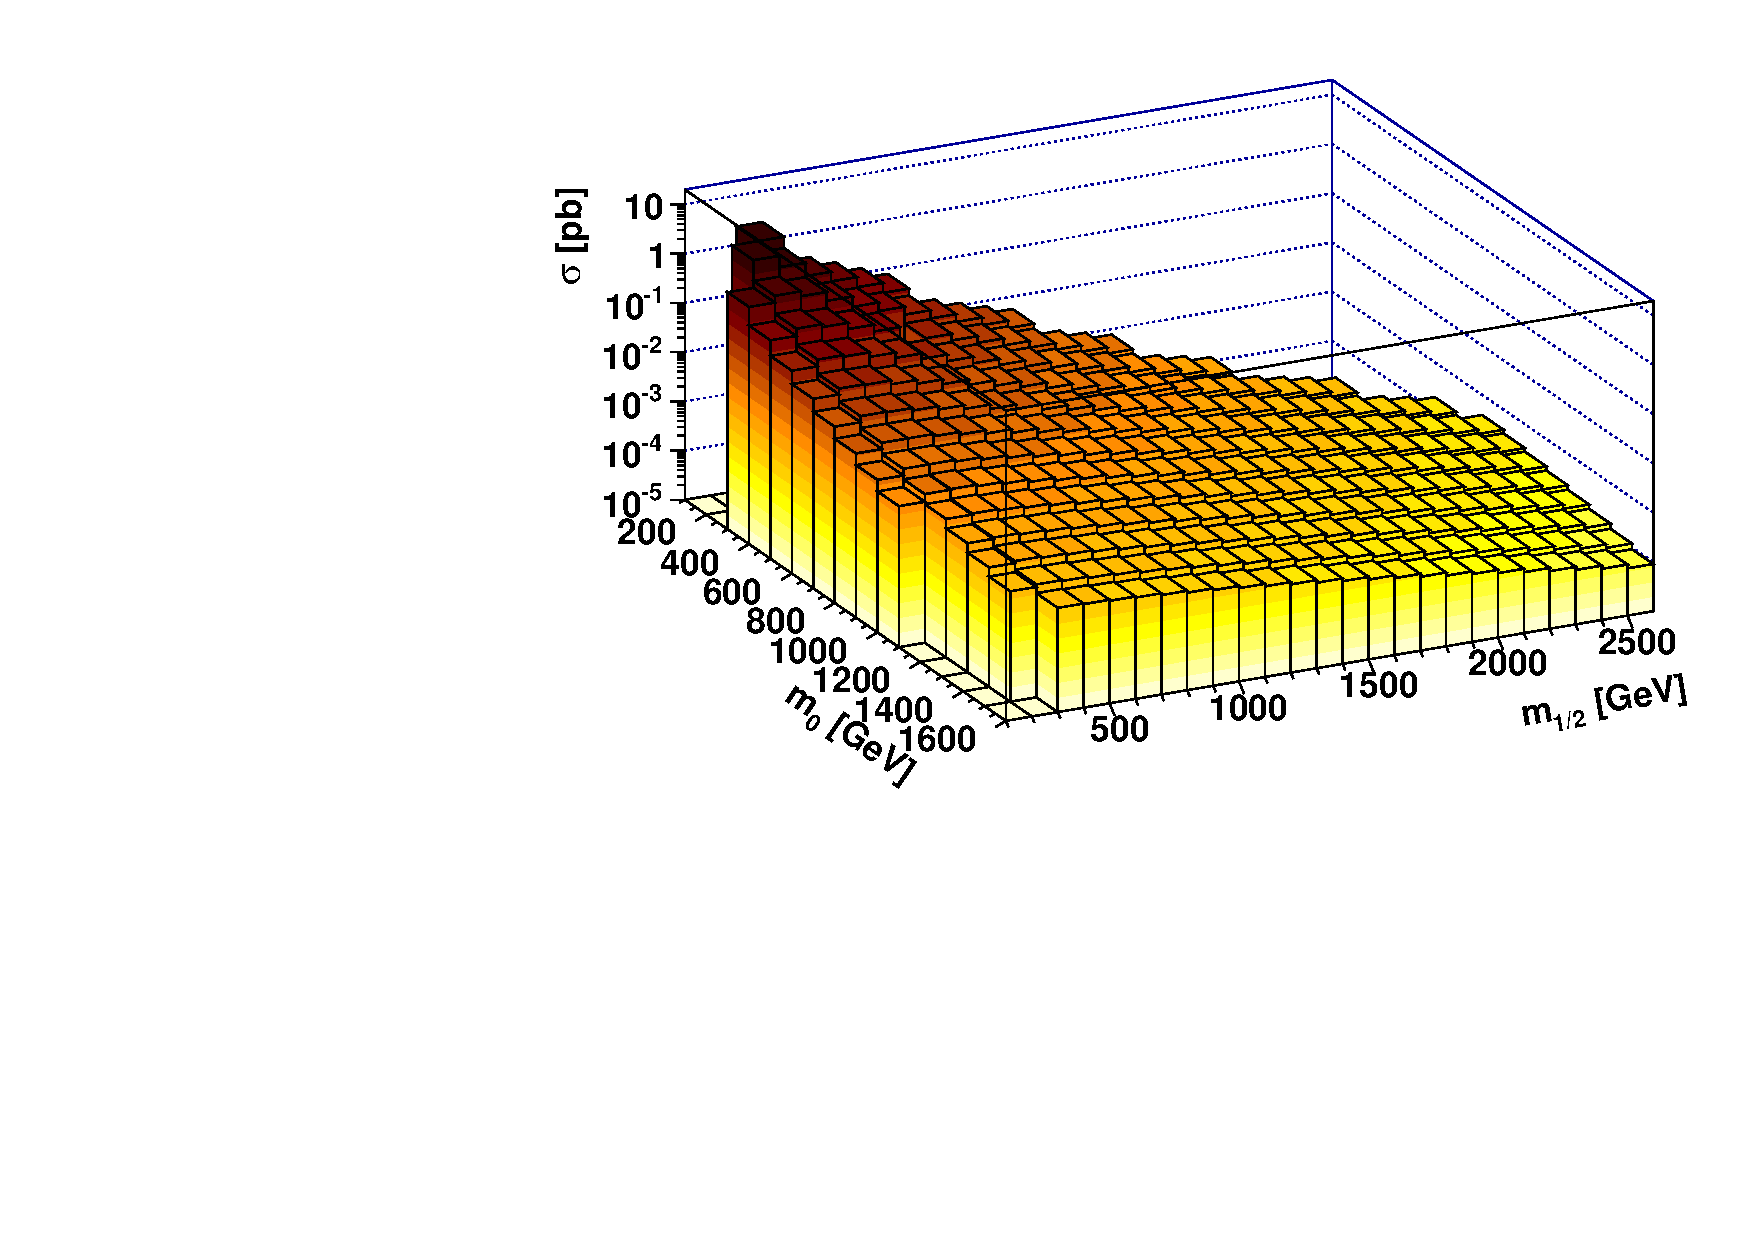
\includegraphics[width=0.6\textwidth]{plots/2dxs.pdf}
  \caption{NLO cross section map for the production of second generation sleptons used in the analysis. The \textit{production} branching fractions of both the smuon and sneutrino have been taking into account for the calculation.}
  \label{fig:susy-2dxs}
\end{figure}

For comparison, three points of the cMSSM parameter phase space will be shown in most of the upcoming distributions. The $m_0 = 300\,\text{GeV}$, $m_{1/2} = 300\,\text{GeV}$ and $m_0 = 1000\,\text{GeV}$, $m_{1/2} = 200\,\text{GeV}$, as well as the $m_0 = 1000\,\text{GeV}$, $m_0 = 1200\,\text{GeV}$ scenario. While the first two are within the range of existing limits (Sec.~\ref{sec:anamodel}), the latter is not. As the corresponding cross sections scale with $\lambda^{\prime\:2}_{211}$, the cross section of the first two scenarios are adjusted to match existing limits. Exemplary distributions displaying the different properties of the signal points are shown in figure~\ref{fig:signal_properties}. Large differences between the distributions of the generated points in phase space can be seen. This is especially apparent in the two muon mass resonances for the smuon and sneutrino While this is expected, it leads to differing efficiencies with regards to certain requirements that are going to be applied in chapter~\ref{cha:eventsel}.

\begin{figure}[!htbp]
  \centering
  \begin{subfigure}[b]{0.495\textwidth}
    \centering
    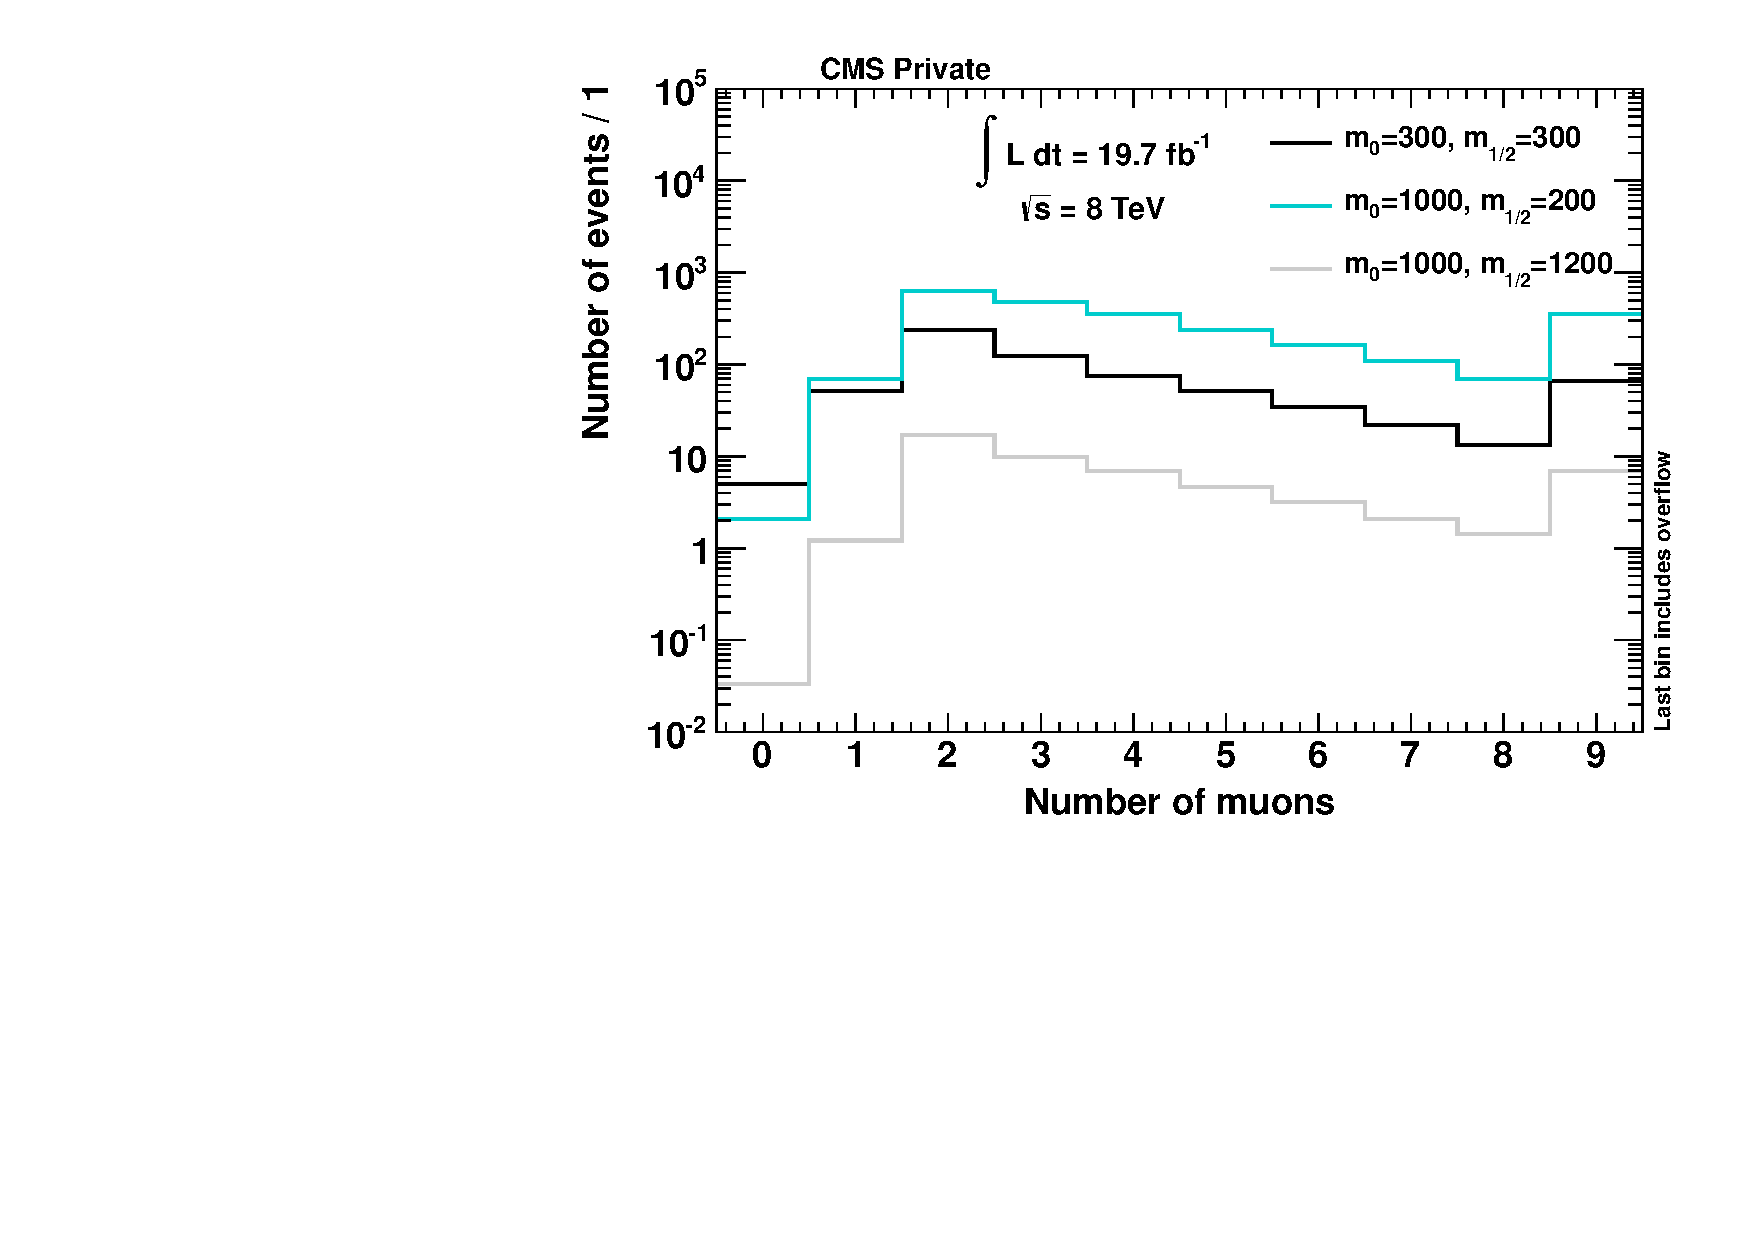
\includegraphics[width=\textwidth]{plots/sig_muo_n.pdf}
    \caption{Number of \textit{reconstructed} muons. $p_{\text{T}, 1\text{st} \mu} > 10\,\text{GeV}$, $p_{\text{T}, \text{st} \mu} > 5\,\text{GeV}$. No further requirements applied.\label{fig:sig_muo_n}}
  \end{subfigure}
  \begin{subfigure}[b]{0.495\textwidth}
    \centering
    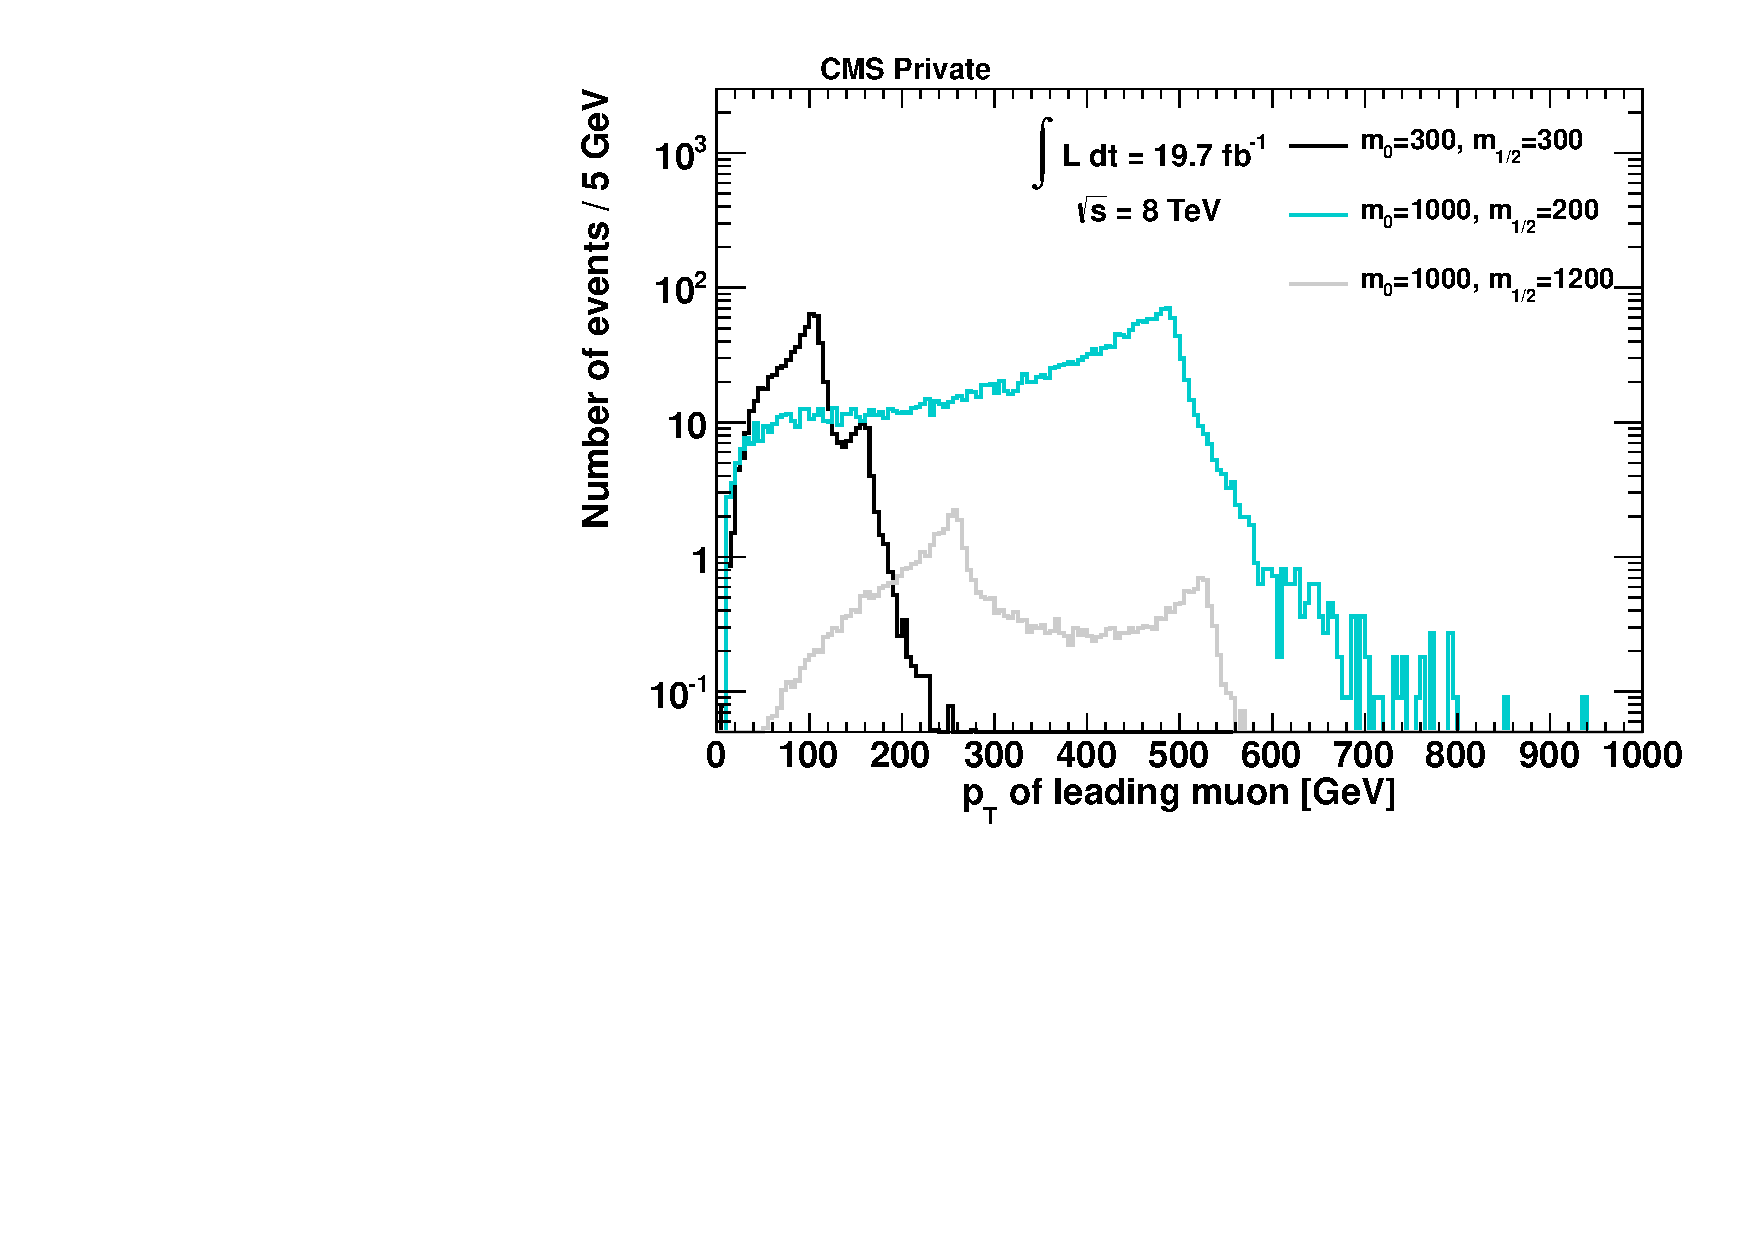
\includegraphics[width=\textwidth]{plots/sig_muo_pt1.pdf}
    \caption{Transverse momentum of leading muon, $p_{\text{T}, 1\text{st} \mu} > 10\,\text{GeV}$. Structures are caused by the smuon and sneutrino\footnotemark.\label{fig:sig_muo_pt1}}
  \end{subfigure}
\end{figure}

\begin{figure}[!htbp]
  \ContinuedFloat
  \centering
  \begin{subfigure}[b]{0.495\textwidth}
    \centering
    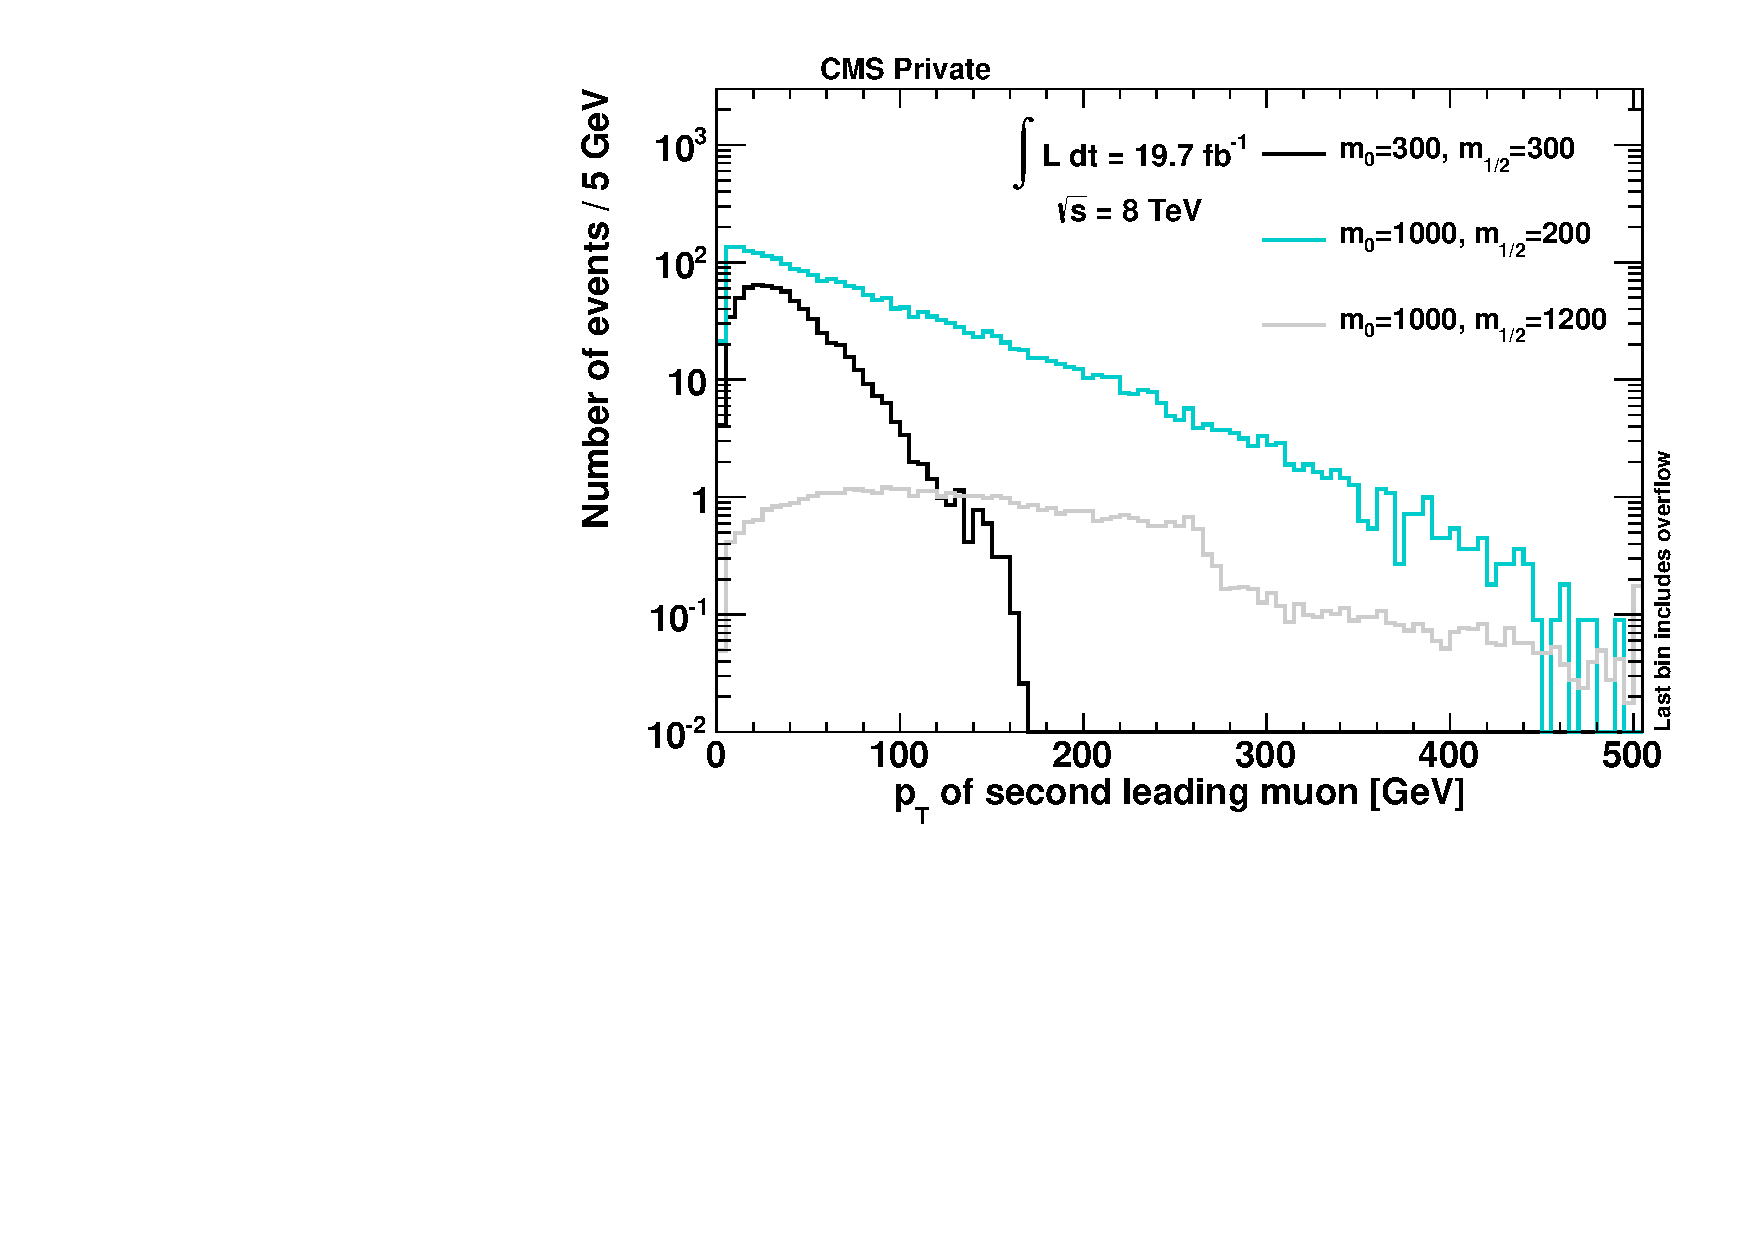
\includegraphics[width=\textwidth]{plots/sig_muo_pt2.pdf}
    \caption{Transverse momentum of sub-leading muon, $p_{\text{T}, \text{st} \mu} > 5\,\text{GeV}$.\label{fig:sig_muo_pt2}}
  \end{subfigure}
  \begin{subfigure}[b]{0.495\textwidth}
    \centering
    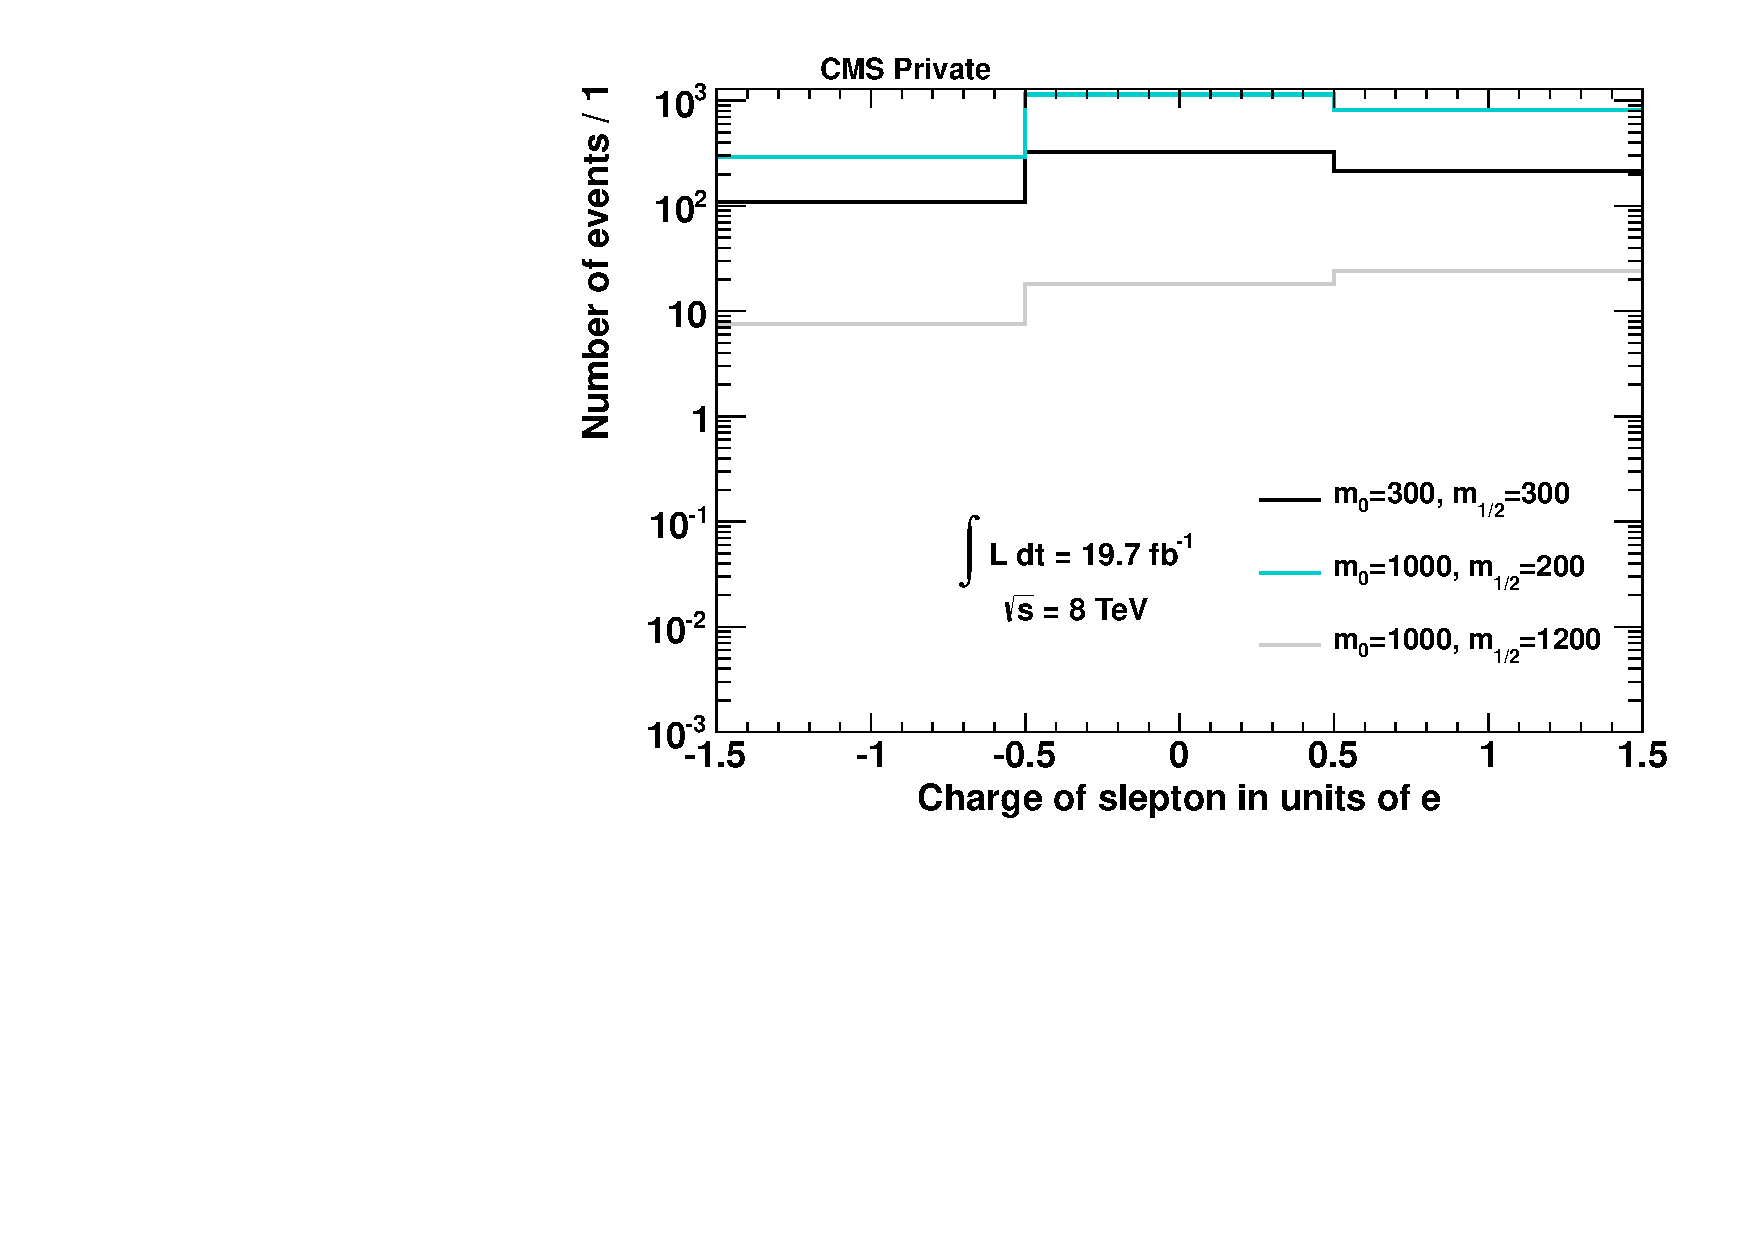
\includegraphics[width=\textwidth]{plots/sig_slepton_charge.pdf}
    \caption{Charge of slepton.\label{fig:sig_slepton_charge}}
  \end{subfigure}
  \caption{Selected properties of the signal Monte Carlo after simulation and reconstruction. For \ref{fig:sig_muo_n} all events passing the generator level filter are included, while for the remaining distributions at least 2 muons and 2 jets per event are required.}
  \label{fig:signal_properties}
\end{figure}

\footnotetext{In the $m_0 = 1000\,\text{GeV}$, $m_0 = 1200\,\text{GeV}$ case, the smuon and sneutrino mass coincide at $m_{\tilde{\nu}} \approx m_{\tilde{\mu}} = 1272\,\text{GeV}$.}

\section{Pileup Reweighting}
\label{sec:pileup}

During 2012 the average number of proton-proton collisions that occured for a single bunch-crossing is 21~\cite{cmslumi}. The distribution for said data taking period is shown in figure~\ref{fig:pileup2012}. However, for the generated Monte Carlo samples the shape differs. Accommodating for that fact is an important step to allow for an accurate simulation of the experiment's conditions.

\begin{figure}[htb!]
  \centering
  \begin{subfigure}[b]{0.495\textwidth}
    \centering
    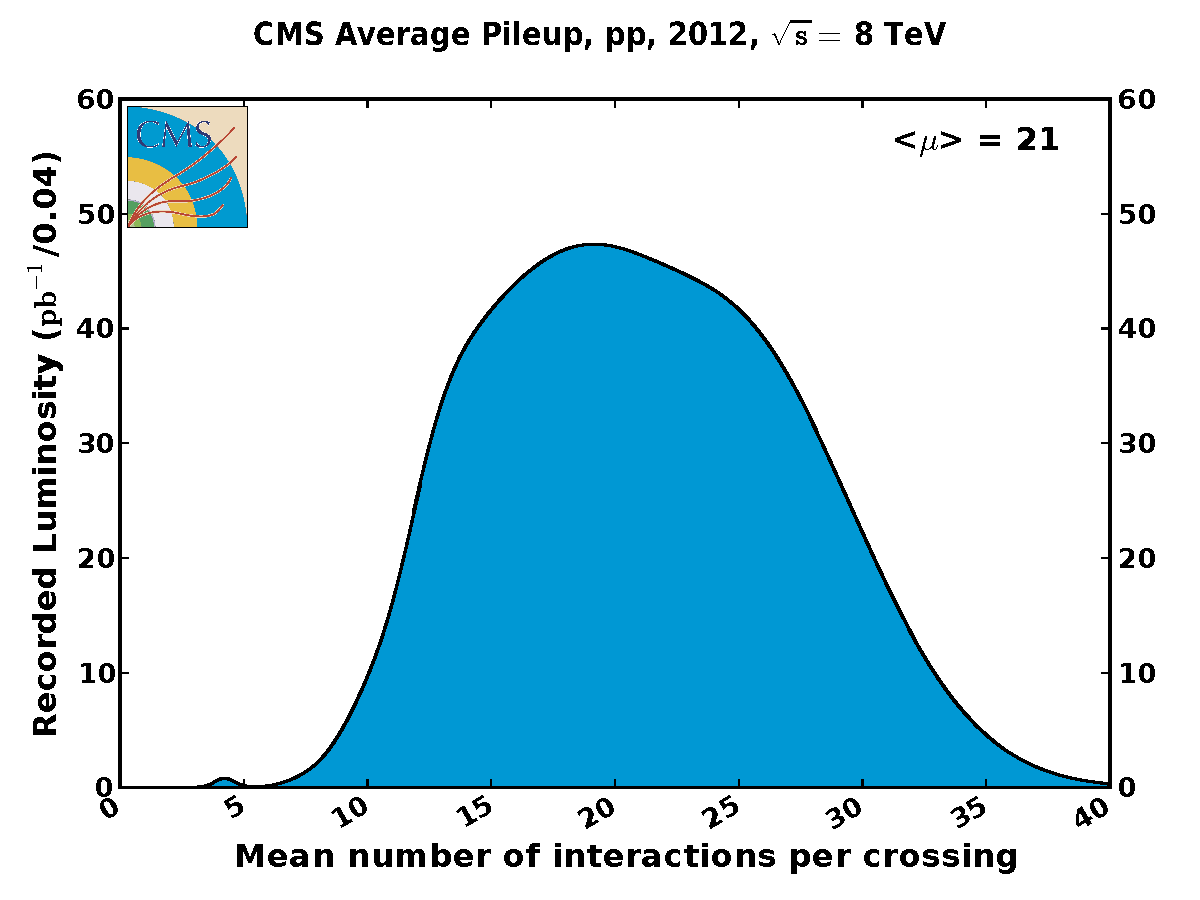
\includegraphics[width=\textwidth]{plots/pileup_pp_2012.pdf}
    \caption{\label{fig:pileup2012}}
  \end{subfigure}
  \begin{subfigure}[b]{0.495\textwidth}
    \centering
    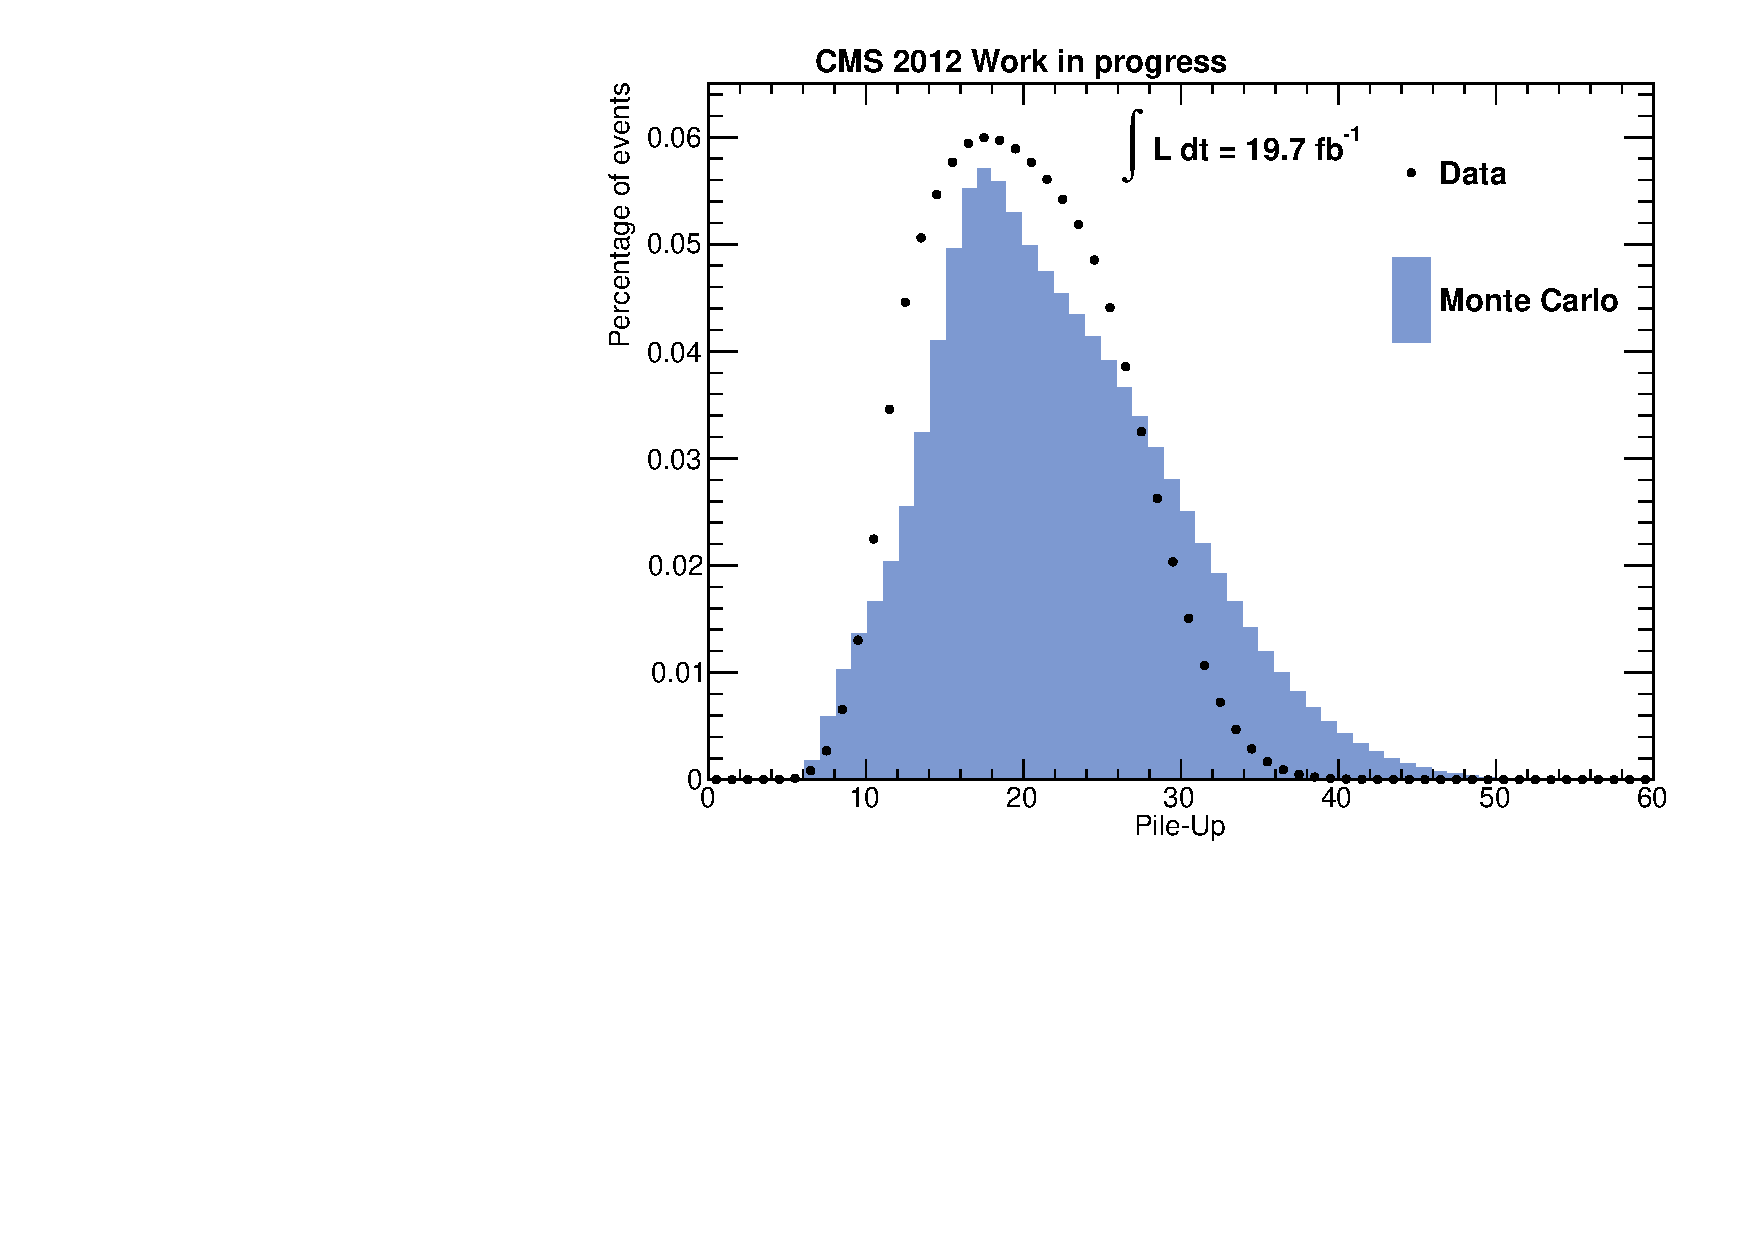
\includegraphics[width=\textwidth]{plots/pileup.pdf}
    \caption{\label{fig:pileup}}
  \end{subfigure}
  \caption{Pileup distribution for the 2012 data taking period (\ref{fig:pileup2012})~\cite{cmslumi} and normalized pileup reweighting distribution (\ref{fig:pileup}).}
  \label{fig:pileups}
\end{figure}

To obtain the (true) number of interactions for each crossing, the instantaneous bunch-by-bunch luminosities are used as input. Combined with the total inelastic cross section, which amounts to $69400\,\mu\text{b}$ at $8\,\text{TeV}$~\cite{pileup}, they can be used to calculate the aforementioned expected number of interactions for each lumisection. While said cross section is entered manually into the script, the luminosities are extracted from a centrally maintained pileup file. In this analysis \verb+pileup_JSON_DCSONLY_190389-208686_All_2012_pixelcorr.txt+ has been used, which already includes corrections from the information provided by the pixel detector. Figure~\ref{fig:pileup2012} shows the histogram filled with the expected number of interactions for the 2012 data taking period. Complementary, figure~\ref{fig:pileup} shows the normalized distribution with the corresponding Monte Carlo entries. These bin contents for the simulated samples have also been gathered centrally and are taken from the dedicated TWiki website~\cite{pileupmc}. All samples in question have been produced with the Summer12 S10 scenario (c.f. app.~\ref{cha:mcsamppath}).

From the ratio of each bin a weight can be calculated and applied to the MC samples on an event by event basis for the analysis. Figure~\ref{fig:vtxn} provides a visualization of the effect of the reweighting.

\begin{figure}[htb!]
  \centering
  \begin{subfigure}[b]{0.495\textwidth}
    \centering
    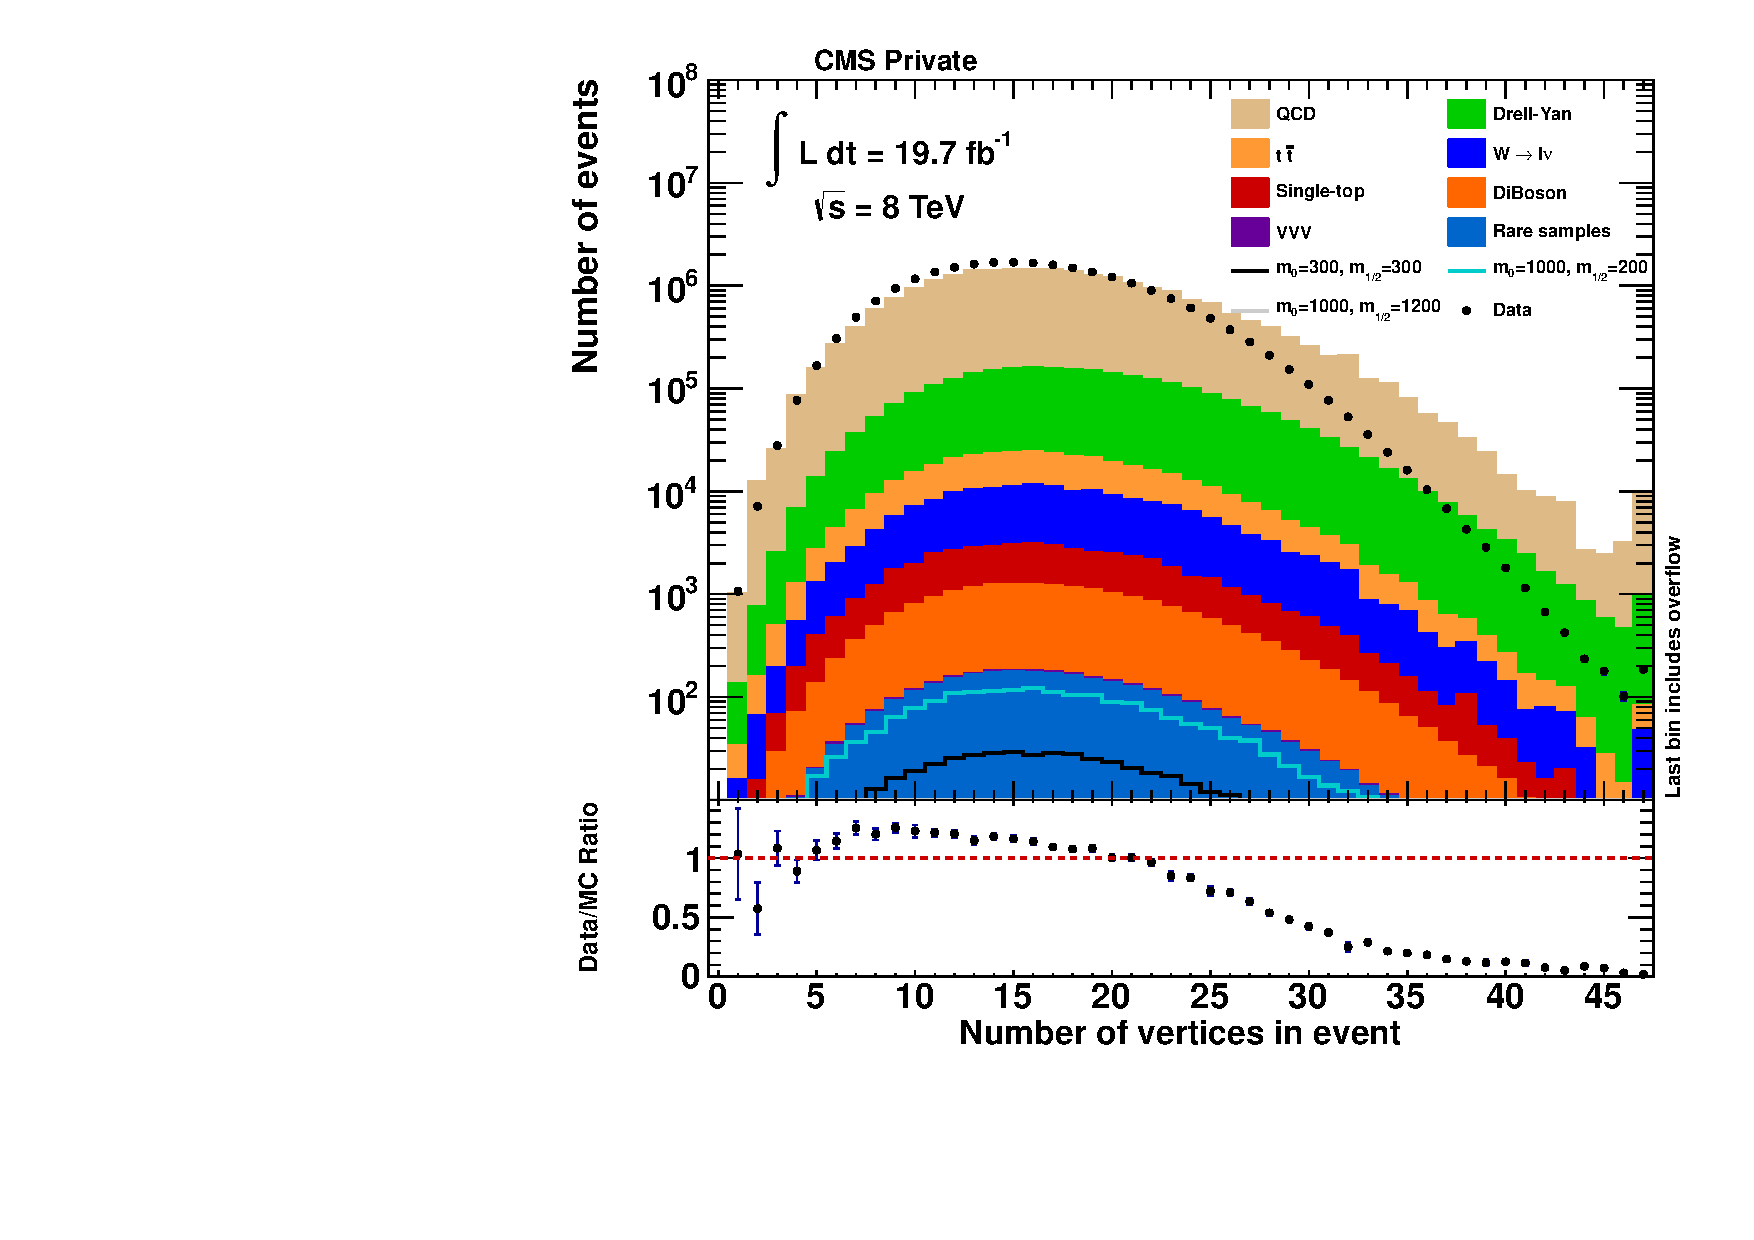
\includegraphics[width=\textwidth]{plots/vtx_n_nopu.pdf}
    \caption{\label{fig:vtx_n_nopu}}
  \end{subfigure}
  \begin{subfigure}[b]{0.495\textwidth}
    \centering
    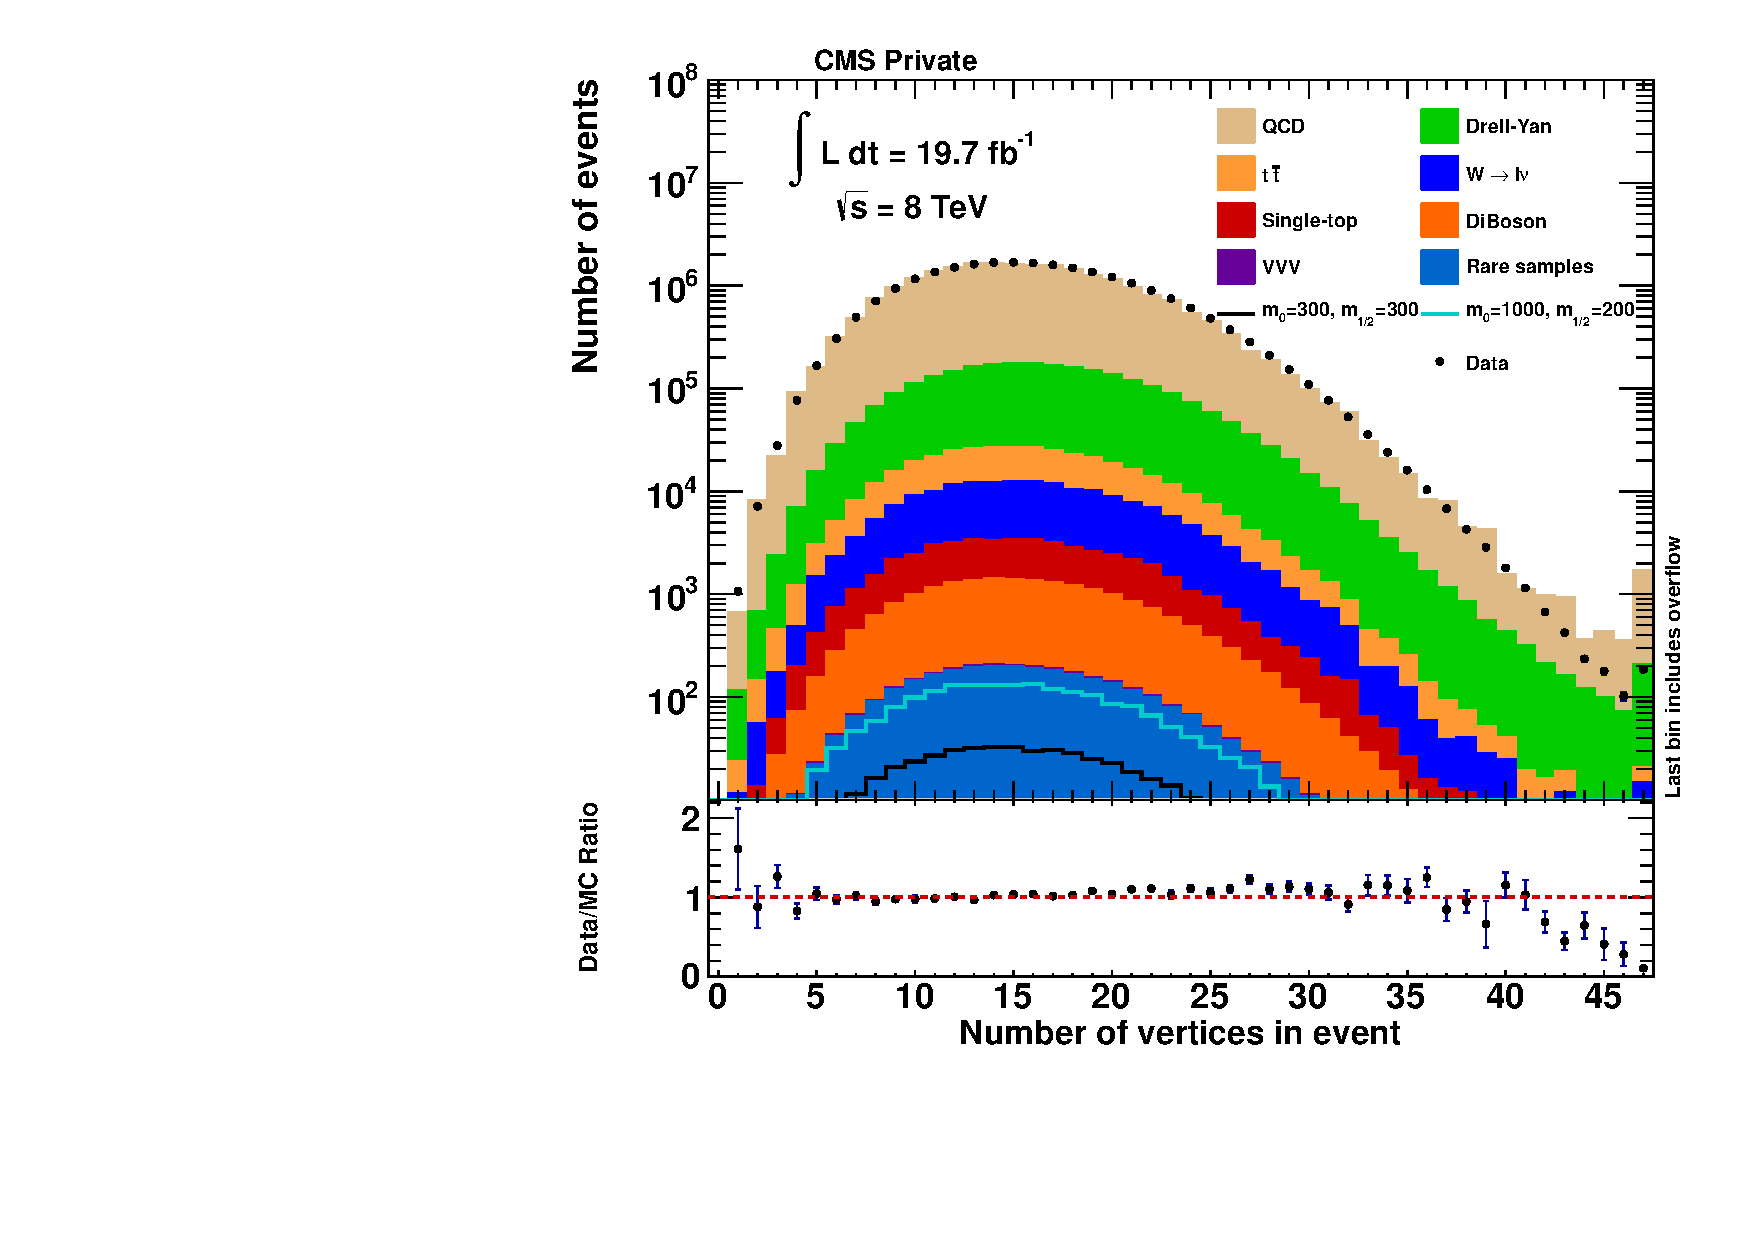
\includegraphics[width=\textwidth]{plots/vtx_n.pdf}
    \caption{\label{fig:vtx_n}}
  \end{subfigure}
  \caption{Number of vertices with (\ref{fig:vtx_n}) and without (\ref{fig:vtx_n_nopu}) pile-up corrections applied to the MC. At this stage of the analysis nothing but the correct trigger (Sec.~\ref{sec:trigger}) and two muons with $p_{\text{T, 1st }\mu} > 10\,\text{GeV}$ are required.}
  \label{fig:vtxn}
\end{figure}

\noindent The distributions are from an early stage of the analysis, where nothing but the correct trigger (Sec.~\ref{sec:trigger}) and two muons with $p_{\text{T, 1st }\mu} > 10\,\text{GeV}$ are required. They show the number of vertices before (Fig.~\ref{fig:vtx_n_nopu}) and after (Fig.~\ref{fig:vtx_n}) the introduction of the weights. With such low requirements and consequently high statistics, the demonstrated improvement is displayed at its greatest impact. Additionally, this is also where the weights are introduced in the analysis. It is important to note that data and simulation are not expected to be in good agreement yet, as showcased by the discrepancies for large numbers of vertices. Nonetheless the histograms display the necessity of this procedure.


\section{Jet Energy Resolution}
\label{sec:jer}

With two jets and no missing transverse energy in the final state, the hadronic calorimeter contributes vital information. However, similarly to the pileup situation, the conditions of the simulation differ from the actual measurement. The energy resolution of the calorimeter is known to be estimated to be too good in the detector simulation~\cite{jer}. To gain access to the resolution, the objects after the simulation stage can be compared to the generator-level ones. Based on this information and the set of measurements the necessary scale factor can be determined.

Every reconstructed particle flow jet above $15\,\text{GeV}$ transverse momentum is considered relevant for the analysis. The algorithm searches for generator-level (\textbf{gen-}) jets in a cone of $\Delta R = \sqrt{\Delta\phi^2 + \Delta\eta^2} = 0.5$ in spatial distance around each reconstructed (\textbf{reco-}) jet. Depending on whether or not any matching objects are found, one of the following two recipes for adjusting the reconstructed jet energy resolution (\textbf{JER}) are used. \\


\textbf{Matched gen-jets:} In case there are matching gen-jets, the formula used to smear the jet energy is given by:
\begin{equation}
  \label{eq:jermatched}
  p^\prime_{\text{T}} = p_{\text{T}, \text{GEN}} + c \cdot (p_{\text{T}} - p_{\text{T}, \text{GEN}})
\end{equation}
  
\noindent The transverse momentum $p_{\text{T}}$ is replaced by a new value $p_{\text{T}}^\prime$, based on the generator information for the transverse momentum $p_{\text{T, GEN}}$. Here $c$ denotes the core resolution scaling factors. To determine those, $0.8\,\text{fb}^{-1}$ of 2011 dijet data\footnote{No significant deviations have been observed with more statistics and 2012 data} have been used~\cite{jer}. The values are given in table~\ref{tab:jerfactors}.

  \begin{table}[htbp!]
    \centering
    {\renewcommand{\arraystretch}{1.2}
      \begin{tabular}{|c|c|}
        \hline
        $\eta$-Range & Ratio of data/MC $\pm$ stat. $\pm$ sys. \\ \hline \hline
        $0.0 < |\eta| < 0.5$ & $1.052 \pm 0.012 ^{+0.062}_{-0.061}$ \\ \hline
        $0.5 < |\eta| < 1.1$ & $1.057 \pm 0.012 ^{+0.056}_{-0.055}$ \\ \hline
        $1.1 < |\eta| < 1.7$ & $1.096 \pm 0.017 ^{+0.063}_{-0.062}$ \\ \hline
        $1.7 < |\eta| < 2.3$ & $1.134 \pm 0.035 ^{+0.087}_{-0.085}$ \\ \hline
        $2.3 < |\eta| < 5.0$ & $1.288 \pm 0.127 ^{+0.155}_{-0.153}$ \\ \hline
      \end{tabular}
    }
    \caption{Core resolution scaling factors $c$ as used for jet energy smearing. They are taken from the JER TWiki~\cite{jer}.}
    \label{tab:jerfactors}
  \end{table}
  
\textbf{No matched gen-jets:} Without a gen-jet match, the jet energy resolution cannot be estimated. Following the official recommendations~\cite{jer}, one can instead randomly smear the \textit{reconstructed} transverse momentum of the jet. The values are assumed to follow a Gaussian distribution with a width of $\sigma = \sqrt{c^2-1} \cdot \sigma_{\text{MC}}$. The core resolution scaling factors $c$ remain the same, but the energy resolution of jets $\sigma_{\text{MC}}$ has to be derived from the Monte Carlo samples. In figure~\ref{fig:jerdeltapt} the difference between the transverse momentum of matched reco- and gen-jets is shown.

\begin{figure}[htb!]
  \centering
  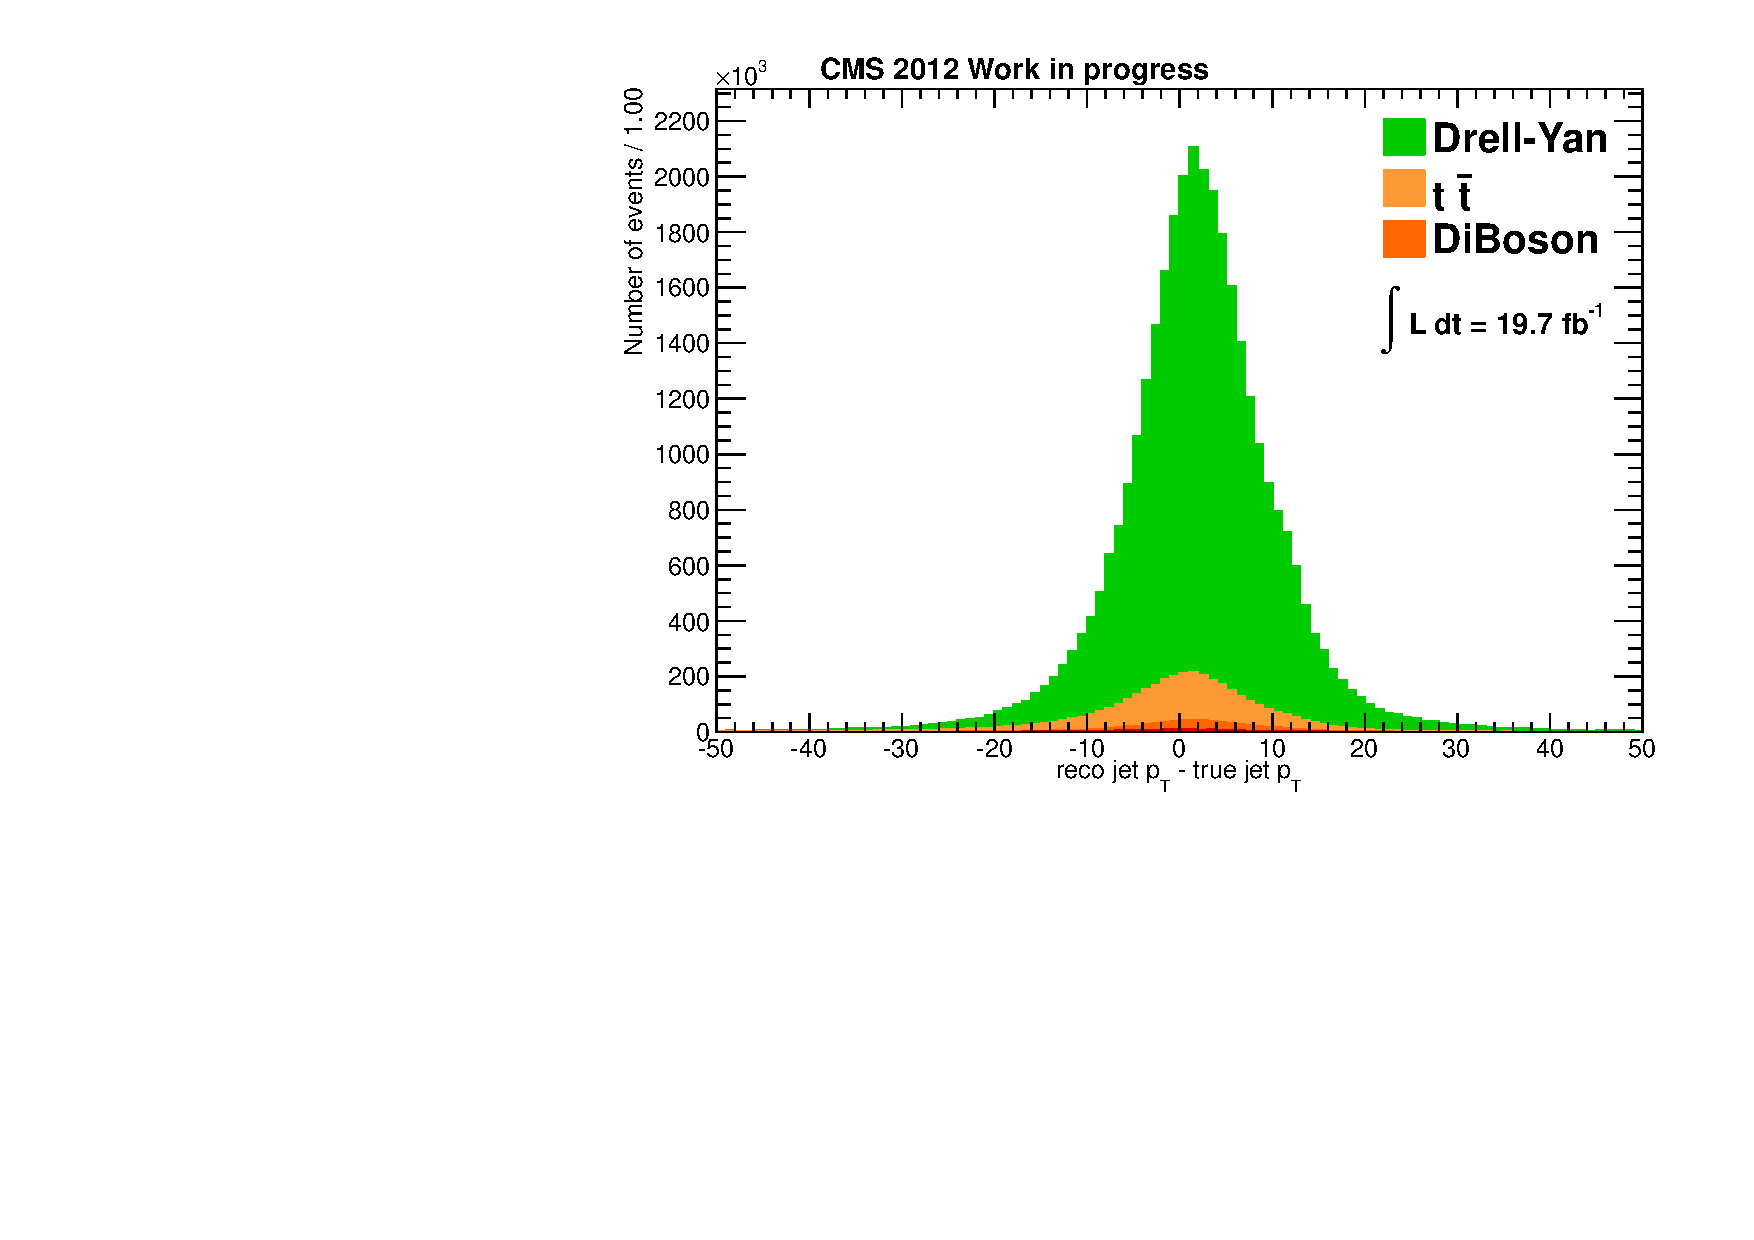
\includegraphics[width=0.6\textwidth]{plots/jer_deltapt.pdf}
  \caption{Difference of transverse momenta from matched reco- and gen-jets in a $\Delta R = 0.5$ cone. This is used to determine the jet energy resolution in the Monte Carlo samples. This histogram is generated after applying the muon quality criteria (Sec.~\ref{sec:muonqualy}), with the analysis being re-run with its result.}
  \label{fig:jerdeltapt}
\end{figure}

\noindent Determining the width of this distribution yields the energy resolution. The entire distribution cannot be accurately modeled with a Gaussian function, however the width of the peak is reasonably well described. It yields $\sigma_{\text{MC}} = 6.2\,\text{GeV}$ a negligible statistical error. While this distribution does depend slighty on the transverse momentum and $\eta$ of the jet, the resolution of the majority of jets is well described by this value. Variations of $\sigma_{\text{MC}}$ have shown an impact of less than $1\,\pct$ on the final distribution. The $p_{\text{T}}$ and $\eta$ dependence, as well the systematic uncertainty of the fit due to the shape are taken into account in the dedicated systematics section (Sec.~\ref{sec:jersys}).

The correction to the transverse momenta is propagated to the $x$ and $y$ momenta, energy and the missing transverse energy measurements. In figure~\ref{fig:jermet} the particle flow missing transverse energy is shown with and without the correction. Due to the adjustment being expected to be comparatively small, the histogram has been filled before the missing transverse energy requirement (Sec.~\ref{sec:met}) of the analysis. This ensures a reasonable agreement between data and simulation prior to examining the effect of the jet energy resolution.

\begin{figure}[htb!]
  \centering
  \begin{subfigure}[b]{0.495\textwidth}
    \centering
    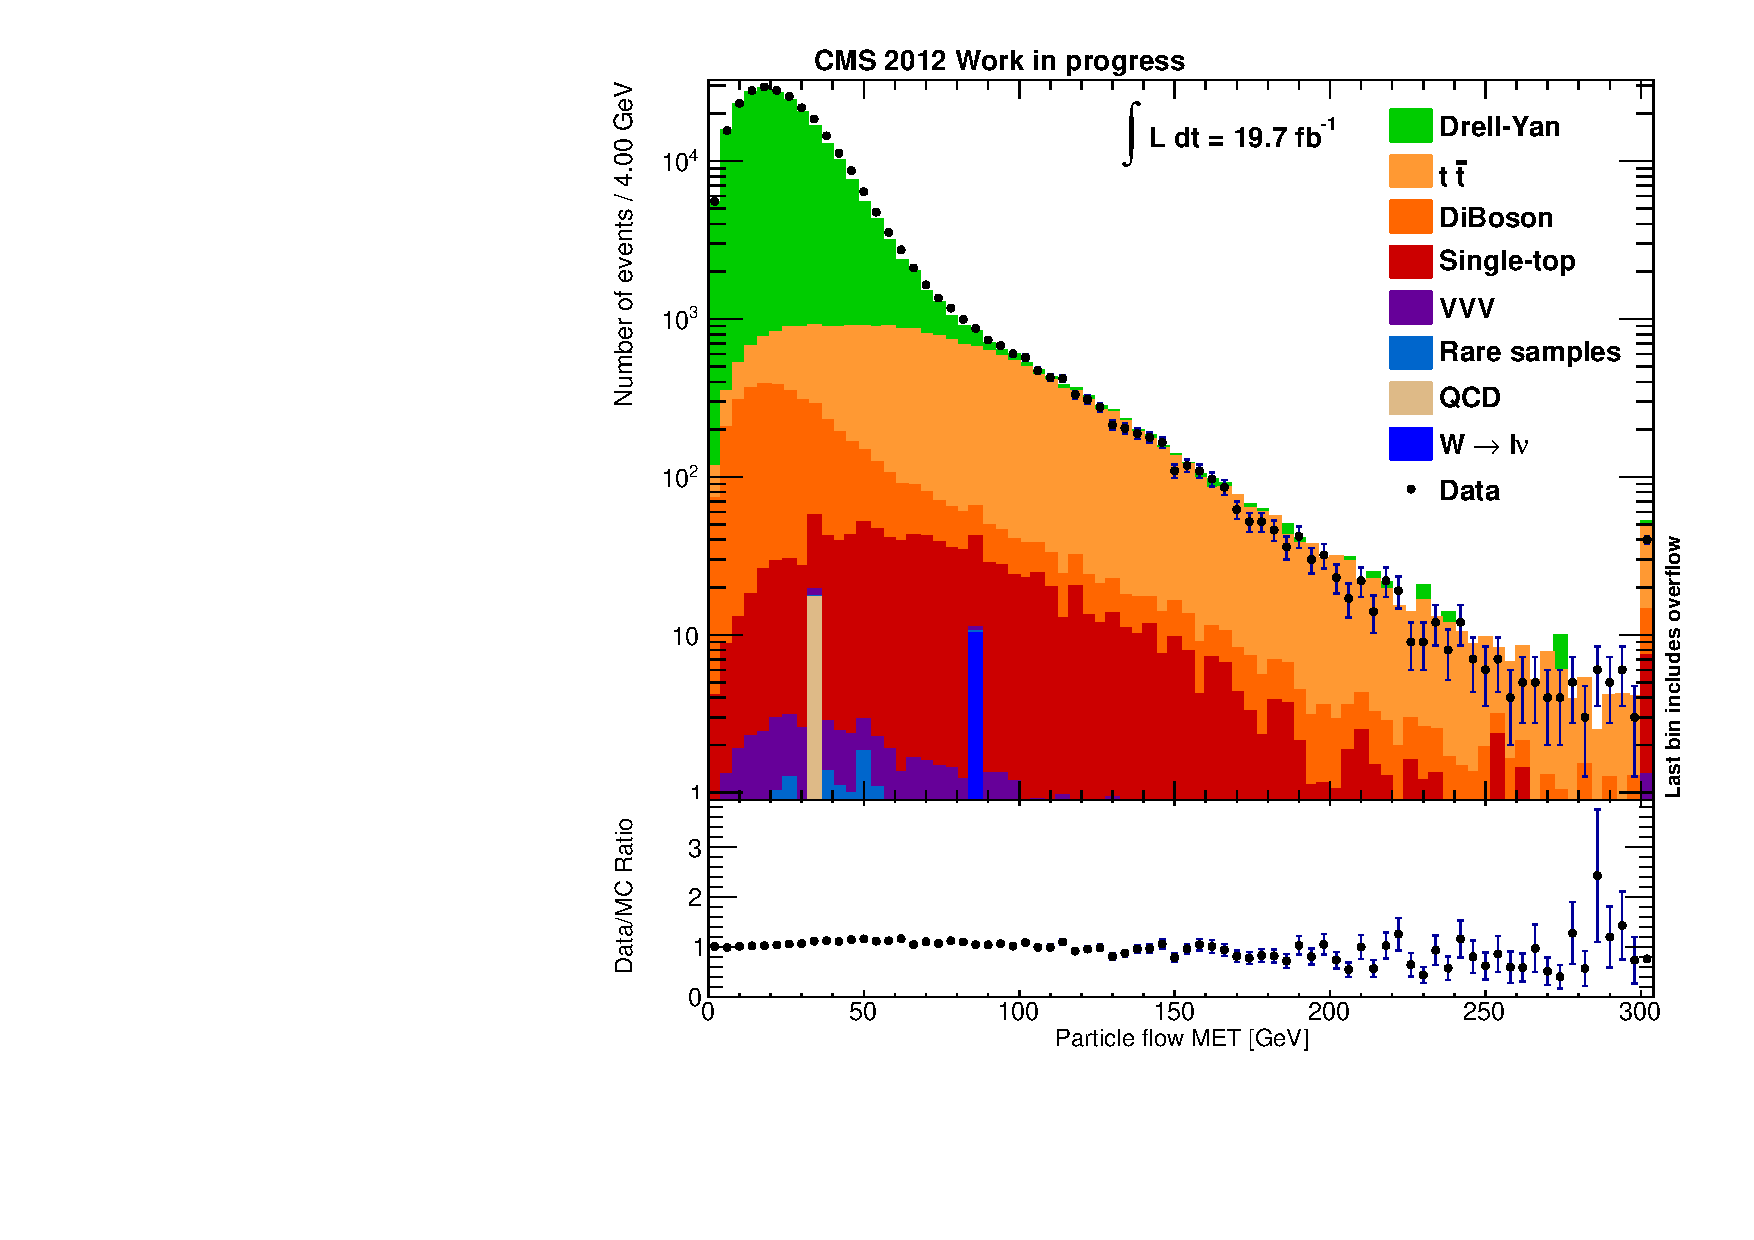
\includegraphics[width=\textwidth]{plots/pfmet_nojer.pdf}
    \caption{\label{fig:jerpfmet_nojer}}
  \end{subfigure}
  \begin{subfigure}[b]{0.495\textwidth}
    \centering
    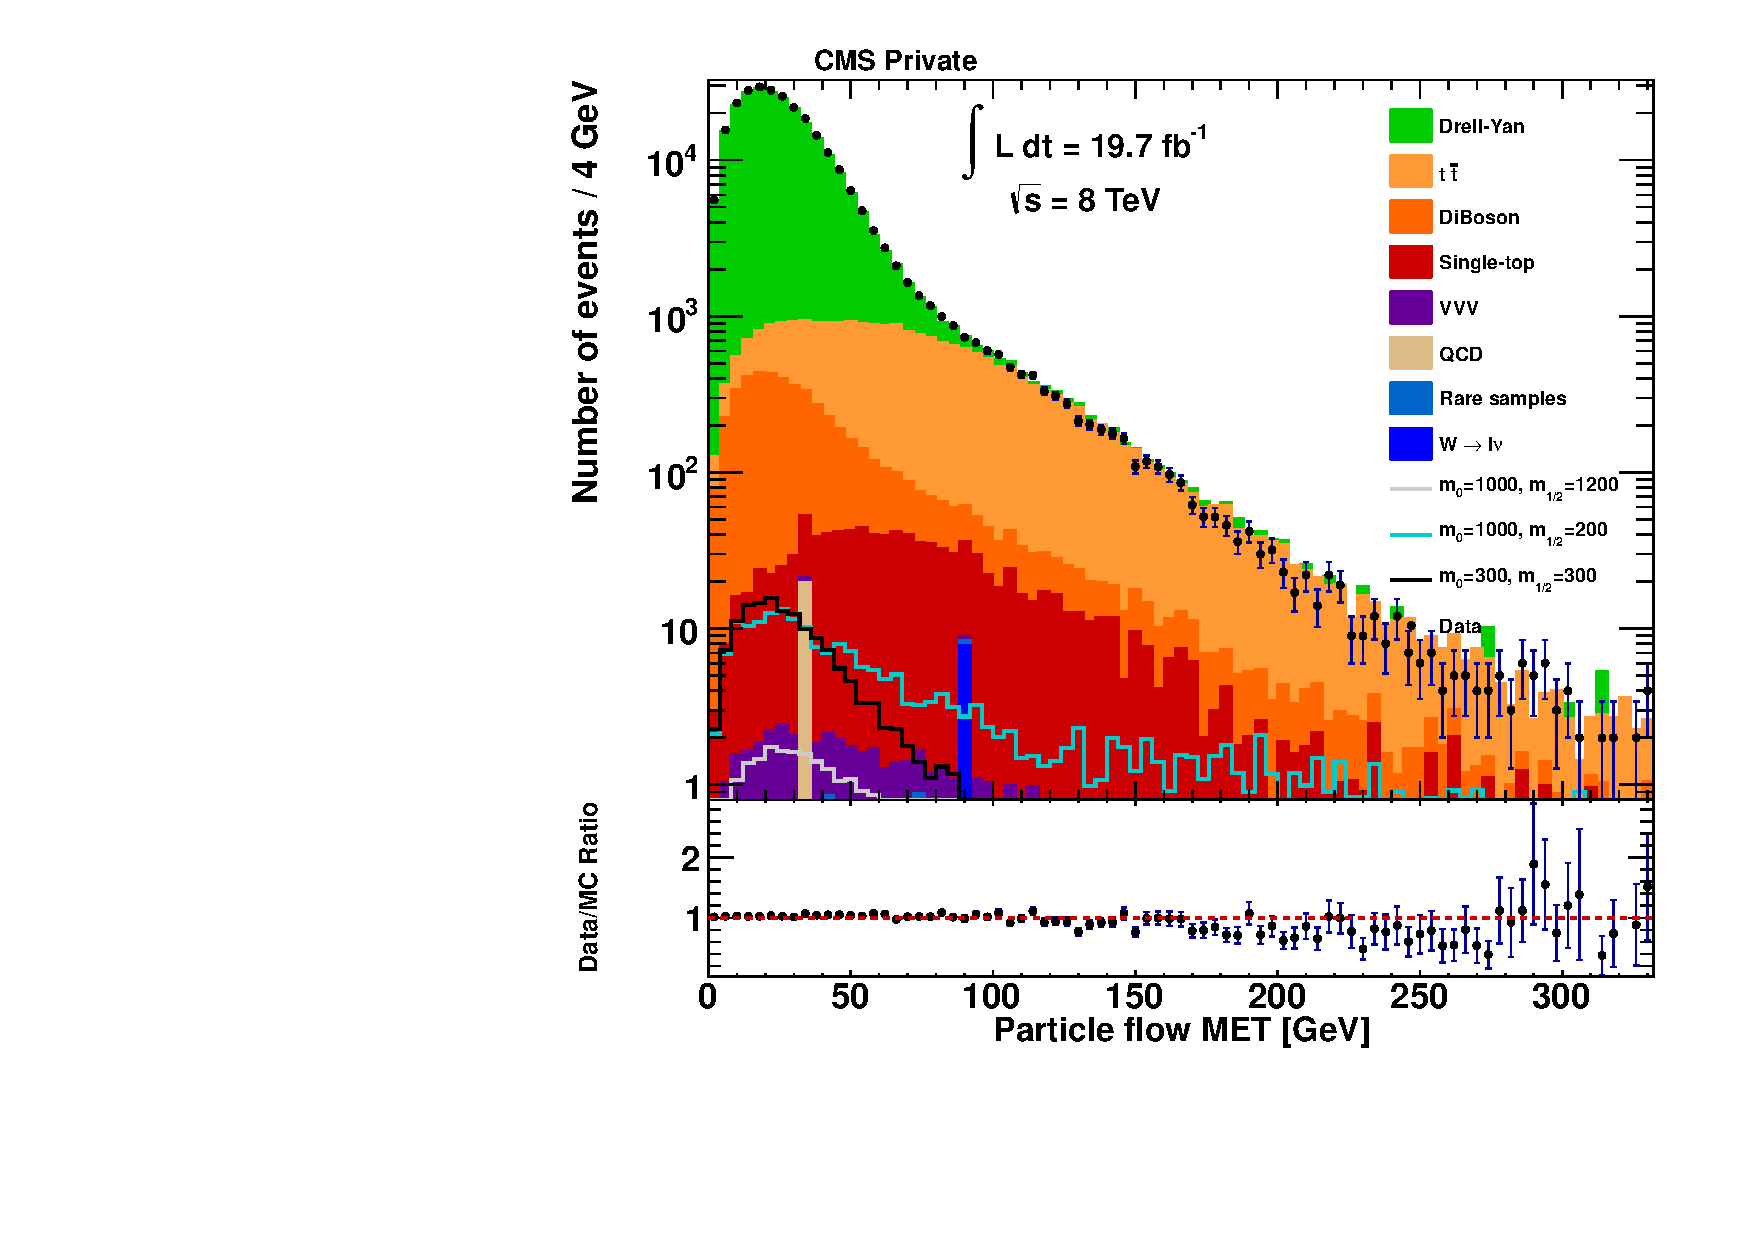
\includegraphics[width=\textwidth]{plots/pfmet.pdf}
    \caption{\label{fig:jerpfmet}}
  \end{subfigure}
  \caption{Particle flow missing transverse energy with (\ref{fig:jerpfmet}) and without jet energy corrections (\ref{fig:jerpfmet_nojer}). Both distributions are composed before the missing transverse energy requirement (Sec.~\ref{sec:met}).}
  \label{fig:jermet}
\end{figure}

\noindent One can observe a small, but still noticeable improvement due to the correction. This is best visible on the right flank of the distribution, where the Drell-Yan process still dominates and the size of the MET is dominated by its resolution rather than by true MET due to undetected neutrinos.


%%% Local Variables: 
%%% mode: latex
%%% TeX-master: "document"
%%% End: 
